\chapter{Monitoring the position of the VELO}
\label{chp:pos_VELO}
%\epigraph{With him it is standing on its head. It must be turned right side up again, if you would discover the rational kernel within the mystical shell.}{\textit{Karl Marx} on Hegel}
Le statistiche ad alto rate mi permettono di monitorare queste quantità. 
Le stesse statistiche le posso anche applicare per monitorare l'allineamento del detector. 

High level processing of low-rate data vs Low-level processing of data at high rate.

Detector levelling 

The low-level statistics at high rate given by the VELO cluster counters have proven to be an efficient estimator for the monitoring of the luminous region as described in Chapter \ref{chap:beamline}. By leveraging PCA on the 208 cluster counters, we have developed a technique to estimate the position of the luminous region with respect to the VELO. The same low-level quantities (i.e. the cluster counters) can be used to perform other monitoring tasks, such as the position of the VELO detector. As explained in Section \ref{sec:velo}, this vertex locator is made of two separate halves that move independently one from the other. This movement is particularly necessary at the start of each physics fill. Since the VELO is installed directly in the beampipe, it is kept at a safe distance from the nominal beamline position until stable beams are declared. Once this condition is reached, the VELO halves move in the x direction from the Fully open configuration to a closed ones (displayed in Figure \ref{fig_velo-xy}). The VELO remain closed until the end of Fill where it is opened again as the beams ramp down. Since the two VELO halves are composed of two different mechanical parts, it is not to exclude that there can be movements of the single halves during a Fill. To address this issue, the real-time estimators described in this chapter can be of extreme usefulness. 
Our strategy involves creating six estimators $\hat{x}_A$, $\hat{y}_A$, $\hat{z}_A$, $\hat{x}_C$, $\hat{y}_C$, $\hat{z}_C$, by using the same technique as the one described in the previous chapter. We achieve this by considering only the 104 counters associated with each half of the VELO, computing the weight vectors by ``training" a PCA model on these counters, i.e. estimating a new set of vector of weights $\mathbf{w^j_(1)}$ from the same Monte Carlo simulation used for the estimation of the coefficients of the luminous region position estimators.
In the simulation, we can invert the point of view and assume a fixed luminous region position at $(0,0,0)$~mm, with the VELO opening on one side by the quantities described in the bullets (i), (ii), (iii) of Section \ref{sec:MC}. 


This approach provides a robust and flexible way to track the position of the two VELO separately in real time, offering insight into potential detector misalignments and enabling corrections where necessary. The corrections can be implemented offline by saving the information of the VELO positions, but it is not to exclude that this information could potentially trigger a mechanical movement that aligns automatically the VELO, providing a sort of ``detector levelling", as it is already done with the luminosity. Additionally, the urgency of this approach stems from observed drift in one of the VELO halves, making it imperative to have a reliable method to monitor and correct for misalignments.

Throughout this chapter, we will describe the implementation of these new estimators, detailing the selection of relevant cluster counters, the calculation of the corresponding weight vectors on Monte Carlo leveraging the PCA technique and a calibration performed on real data.

%Finally, we present the drift of the VELO observed in one of the initial fills of 2024, as a test of the estimators performances.


\section{Estimation of the weights on MC}
As shown in Figure \ref{fig:VELO-counters}, the counters are positioned symmetrically throughout the VELO. Particularly, on each VELO station there are 4 counters on each side of the VELO. By selecting only the 104 counters relative to one side of the VELO, we can ``train" a PCA on these counters to perform an estimation of this VELO side position in the $x$, $y$ and $z$ component, assuming a fixed luminous region. This can be done using the same Monte Carlo simulations and the same approach used in the previous chapter. Although the available MC simulations are made shifting the luminous region, in the assumption of a fixed luminous region position, these shifts can be interpreted as a movement of the VELO. By creating 6 different datasets, one for each combination of position $x,y,z$ and VELO side A and C, we can create the 6 estimators $\hat{x}_A$, $\hat{y}_A$, $\hat{x}_C$, $\hat{y}_C$. 

Since the procedure is the same as the one explained in the previous chapter we do not report it once again. There are only two difference to account for:
\begin{itemize}
    \item only the 104 counters of the VELO side $s=$A,C of interest are used for the estimation of the weights $\mathbf{w}^{j,s}_{(1)}$ at different displacement in the $j=x,y,z$ components.
    \item the counters readings used to estimate the scores $\mathbf{t}^{j,s}_{(1)}$ are divided to the quantity $\mu=5.5$, i.e. the average pp collisions in the events of the MC.
\end{itemize}
We report the comparison between the scores $\mathbf{t}^{j,s}_{(1)}$ (divided by $\mu=5.5$) and the relative ``true" position $j=x,y,z$ for each side $s=$A,C of the VELO in the Figures \ref{fig:x_veloA_fit_MC}, \ref{fig:y_veloA_fit_MC}, \ref{fig:z_veloA_fit_MC}, \ref{fig:x_veloC_fit_MC}, \ref{fig:y_veloC_fit_MC}, \ref{fig:z_veloC_fit_MC}. These figures are scatter plot relative to the estimators $\hat{x}_A$, $\hat{y}_A$, $\hat{z}_A$, $\hat{x}_C$, $\hat{y}_C$$, \hat{z}_C$,  vs the true position of the MC respectively.
\begin{figure}
    \centering
    \begin{subfigure}{0.48\textwidth}
    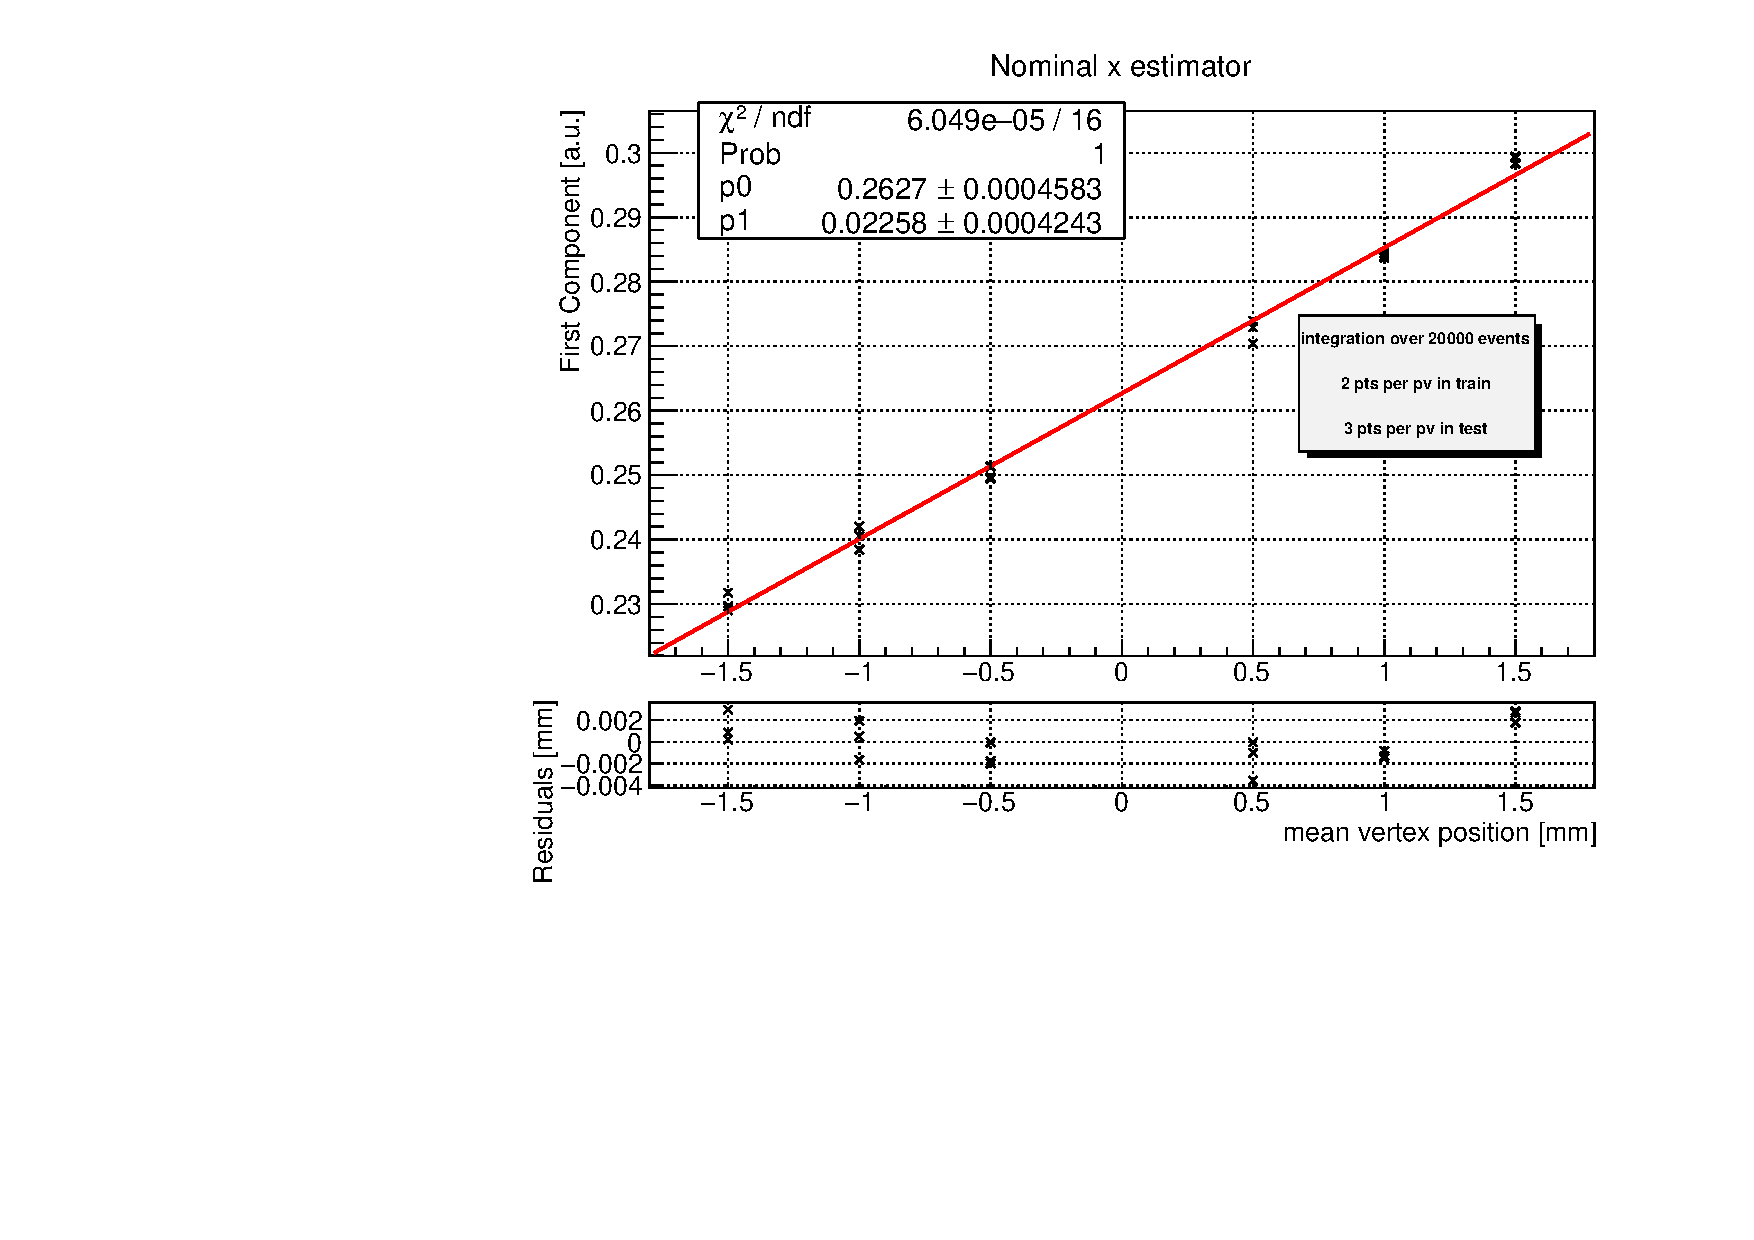
\includegraphics[width=\linewidth]{figures/x_fit_veloA_MC_normalized.pdf}
    \caption{Linear Fit}\label{fig:x_veloA_fit_MC}
    \end{subfigure}
    \begin{subfigure}{0.48\textwidth}
    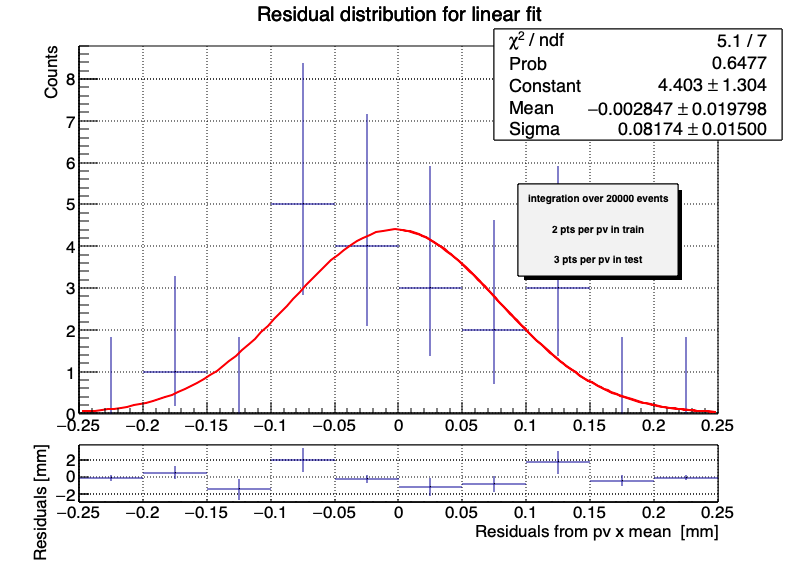
\includegraphics[width=\linewidth]{figures/x_res_veloA_MC.png}
    \caption{Residuals from the fit of the graph on the left. }\label{fig:x_veloA_res_MC}
    \end{subfigure}
    \caption{Linearity of the first component PC divided by $\mu=5.5$ with respect to virtual VELO A position shifts in x component, alongside the residuals distribution fitted with a Gaussian distribution.}
    \label{fig:x_veloA_MC}
\end{figure}


\begin{figure}
    \centering
    \begin{subfigure}{0.48\textwidth}
    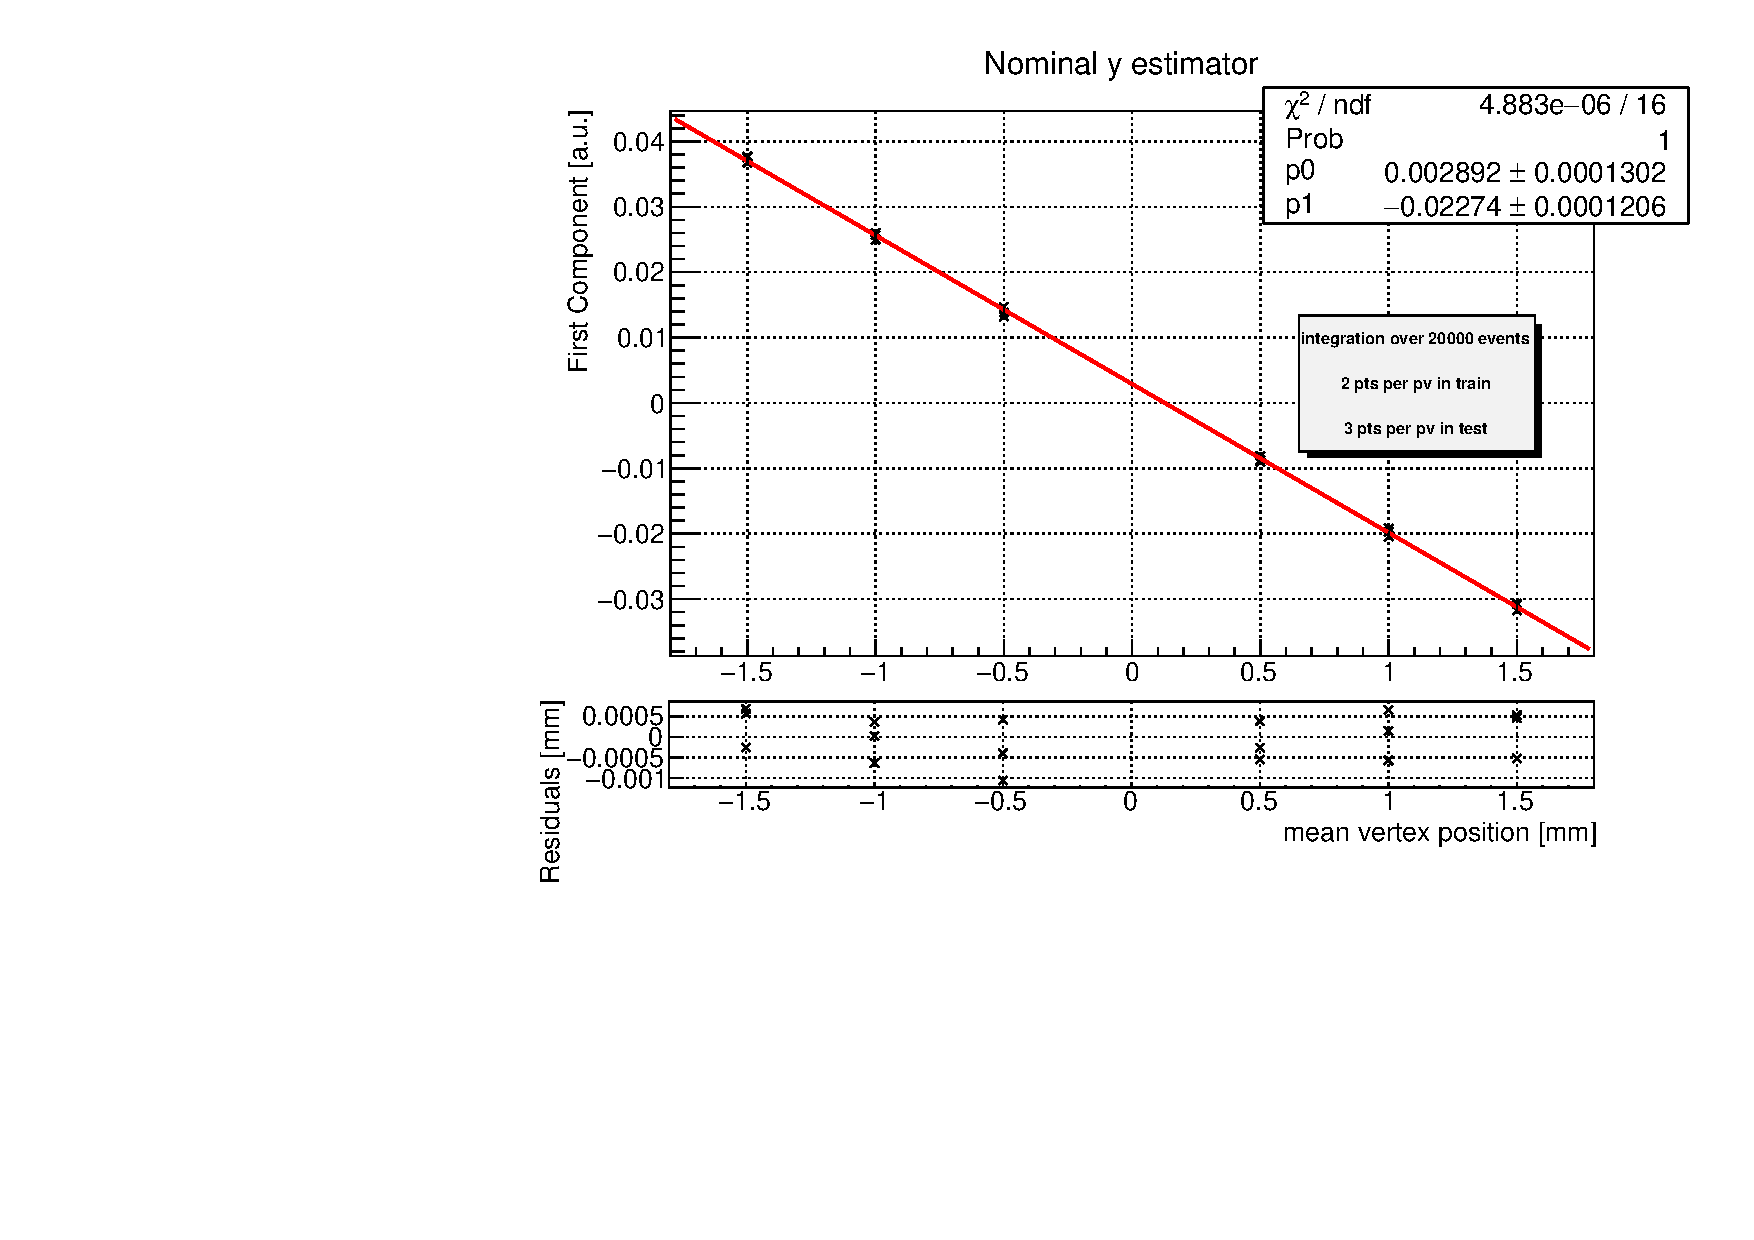
\includegraphics[width=\linewidth]{figures/y_fit_veloA_MC_normalised.pdf}
    \caption{Linear Fit}\label{fig:y_veloA_fit_MC}
    \end{subfigure}
    \begin{subfigure}{0.48\textwidth}
    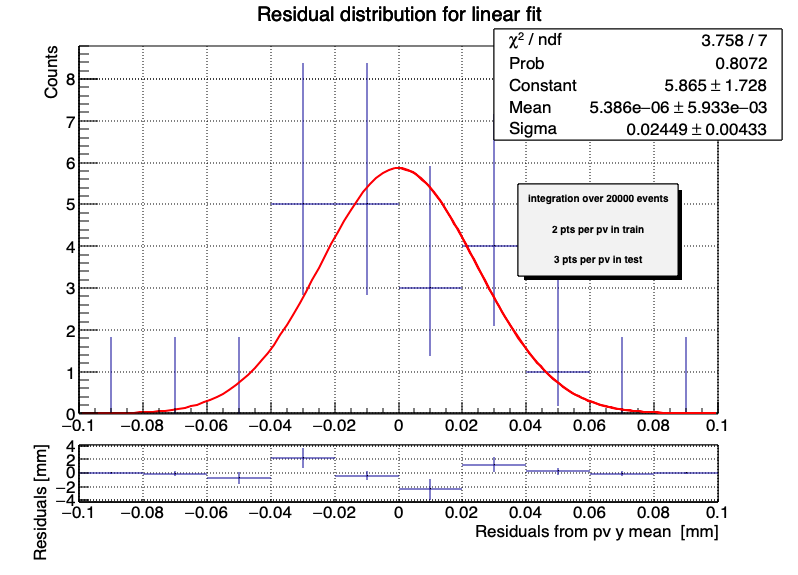
\includegraphics[width=\linewidth]{figures/y_res_veloA_MC.png}
    \caption{Residuals from the fit of the graph on the left. }\label{fig:y_veloA_res_MC}
    \end{subfigure}
    \caption{Linearity of the first PC divided by $\mu=5.5$ with respect to virtual VELO A position shifts in y component, alongside the residuals distribution fitted with a Gaussian distribution.}
    \label{fig:y_veloA_MC}
\end{figure}

\begin{figure}
    \centering
    \begin{subfigure}{0.48\textwidth}
    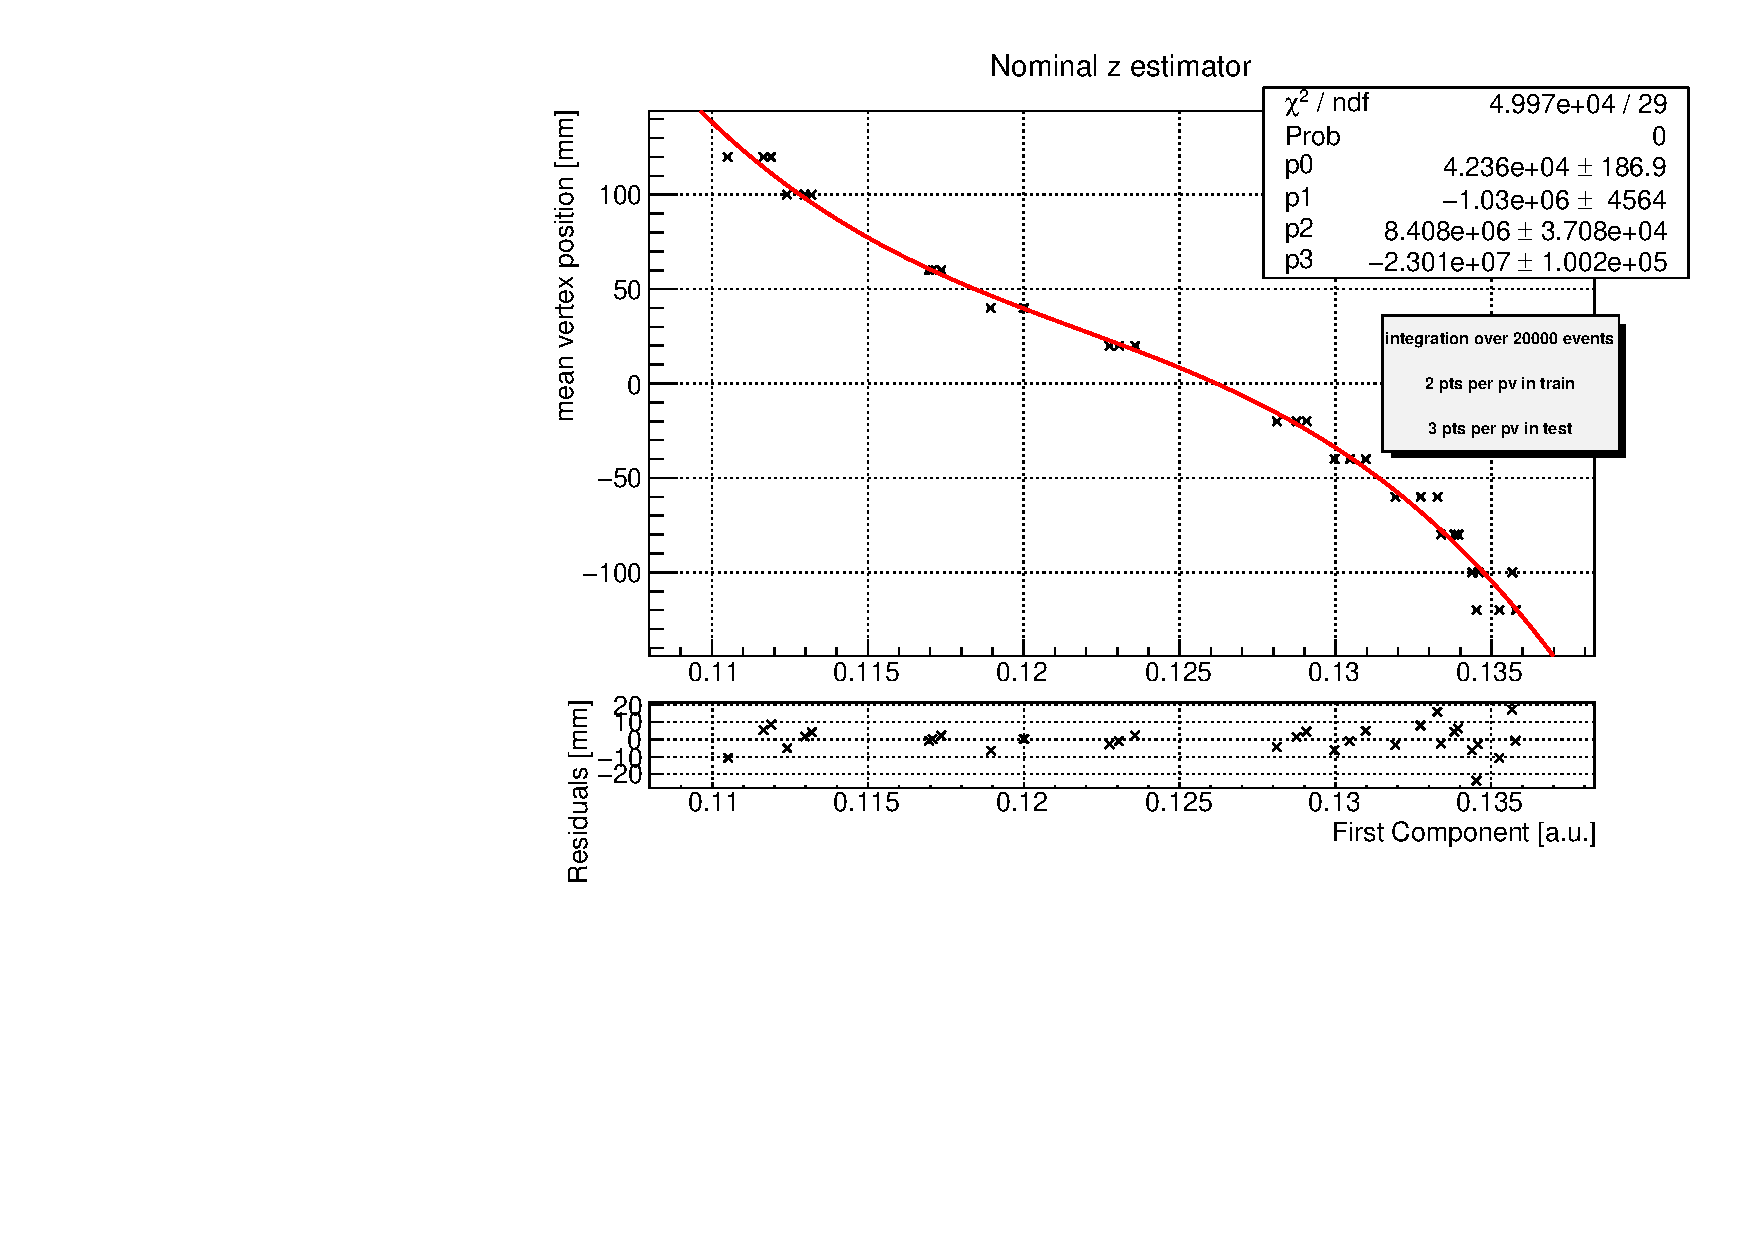
\includegraphics[width=\linewidth]{figures/z_fit_veloA_normalised.pdf}
    \caption{Cubic Fit}\label{fig:z_veloA_fit_MC}
    \end{subfigure}
    \begin{subfigure}{0.48\textwidth}
    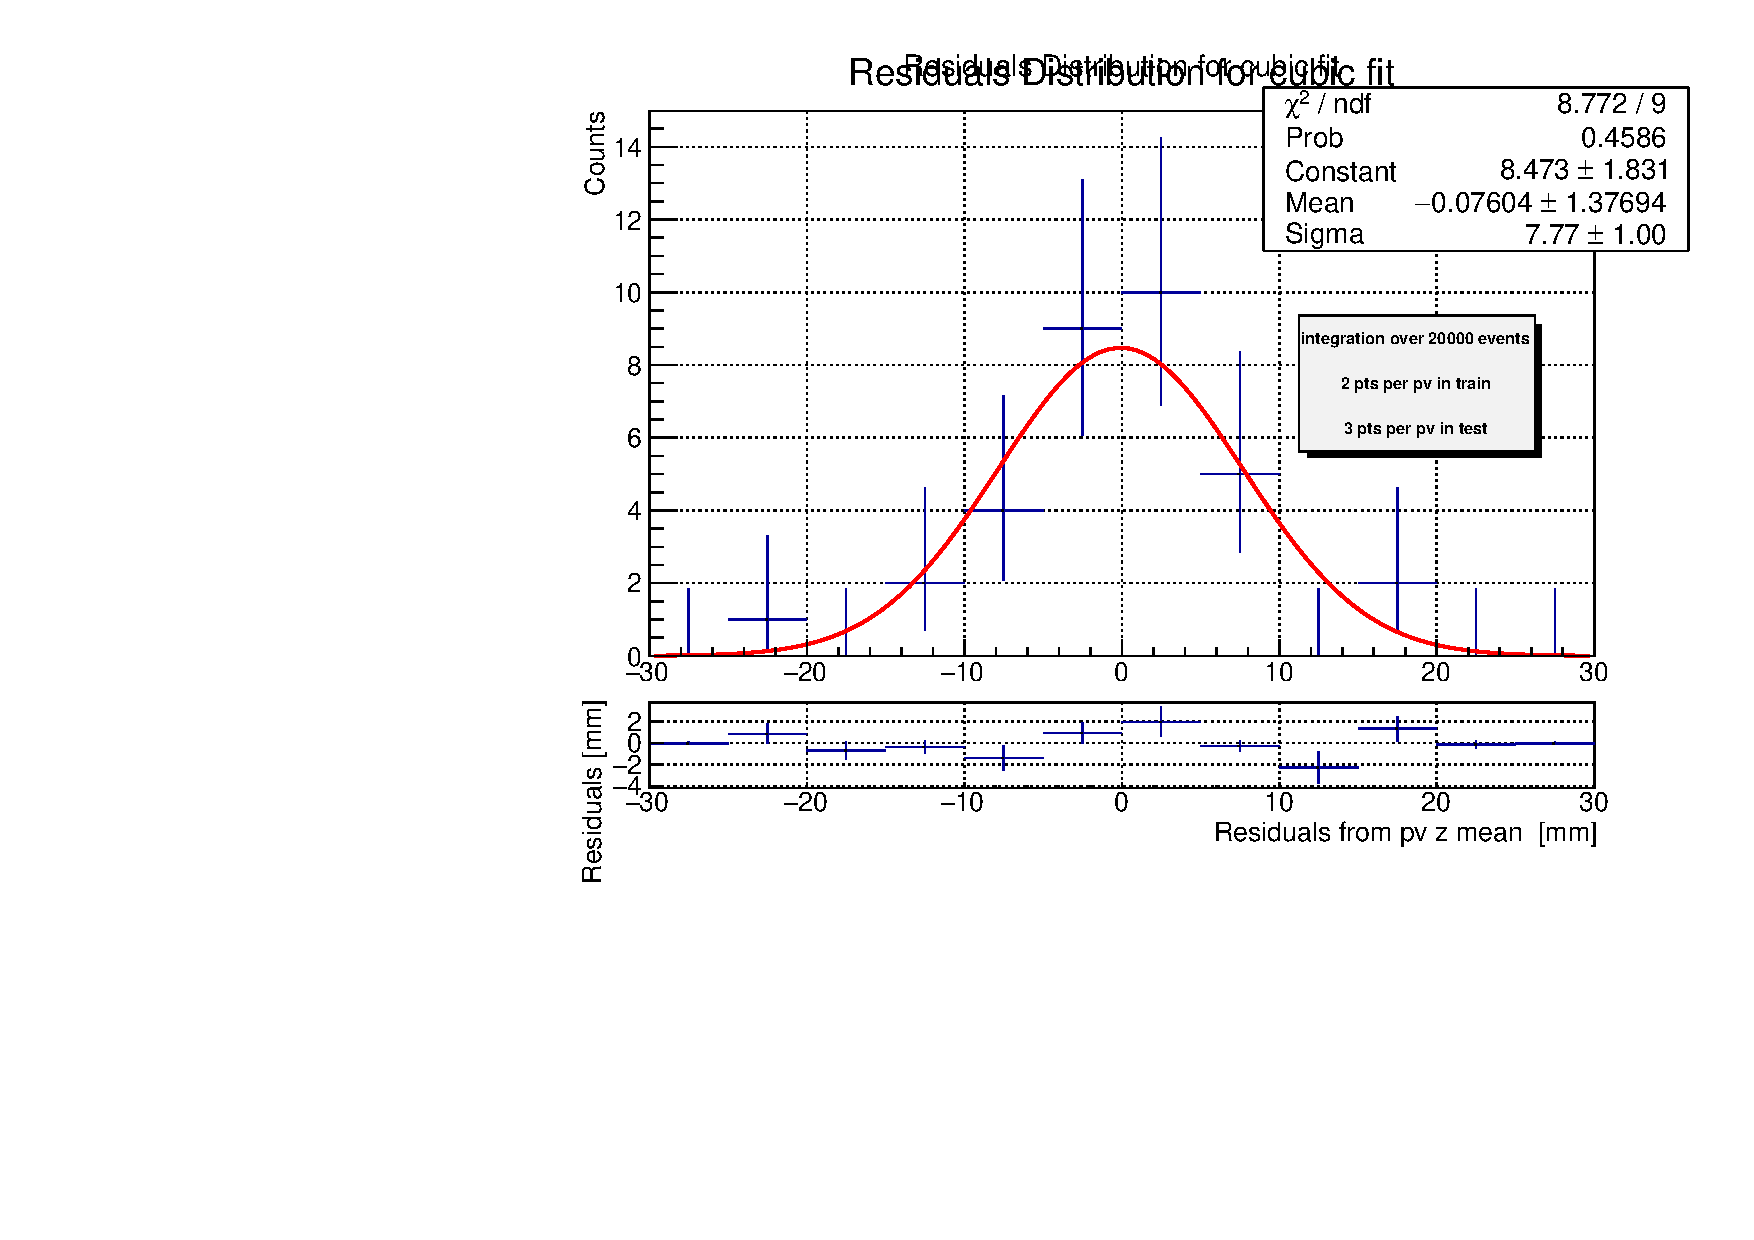
\includegraphics[width=\linewidth]{figures/z_res_veloA_normalised.pdf}
    \caption{Residuals from the fit of the graph on the left. }\label{fig:z_veloA_res_MC}
    \end{subfigure}
    \caption{Cubic relationship of the first PC divided by $\mu=5.5$ with the PCA with respect to virtual VELO A position shifts in z component, alongside the residuals distribution fitted with a Gaussian distribution.}
    \label{fig:z_veloA_MC}
\end{figure}

\begin{figure}
    \centering
    \begin{subfigure}{0.48\textwidth}
    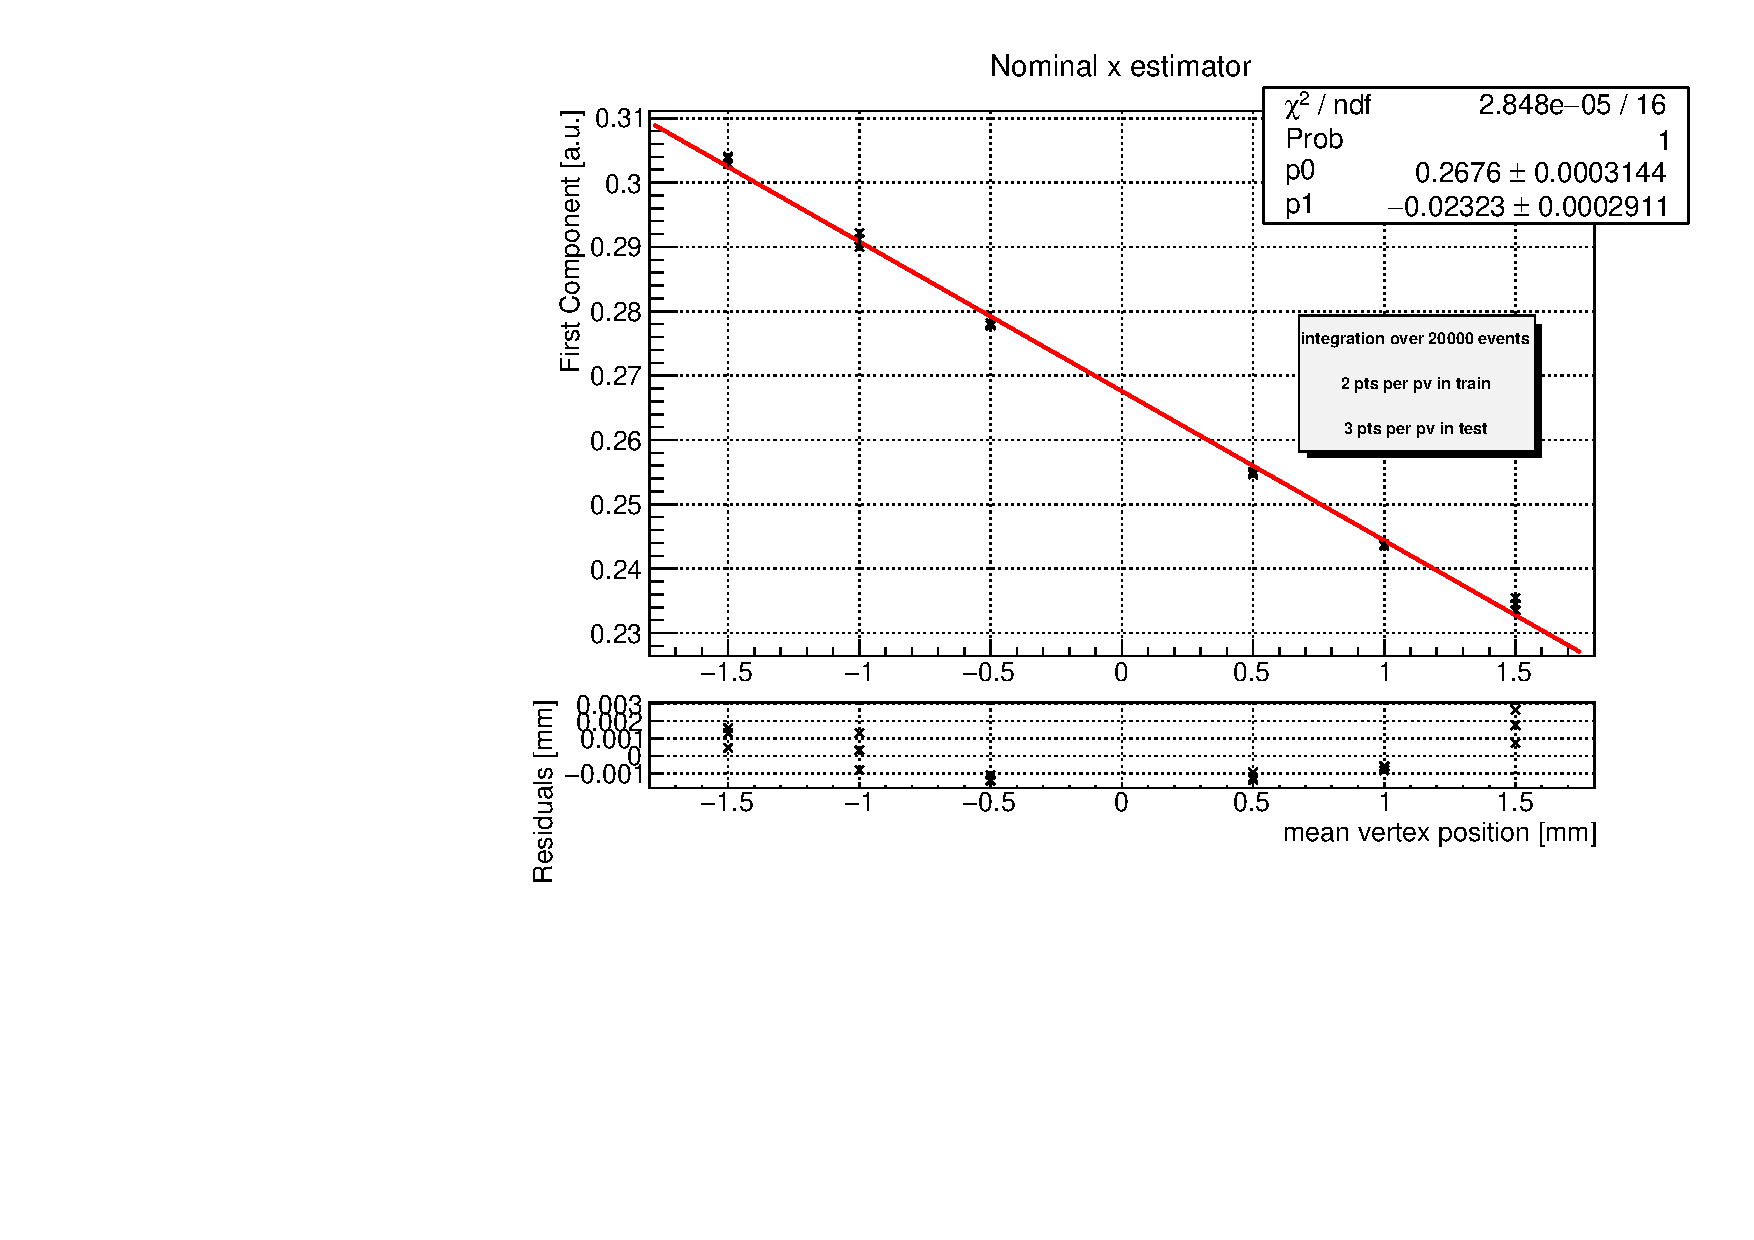
\includegraphics[width=\linewidth]{figures/x_fit_veloC_MC_normalised.pdf}
    \caption{Linear Fit}\label{fig:x_veloC_fit_MC}
    \end{subfigure}
    \begin{subfigure}{0.48\textwidth}
    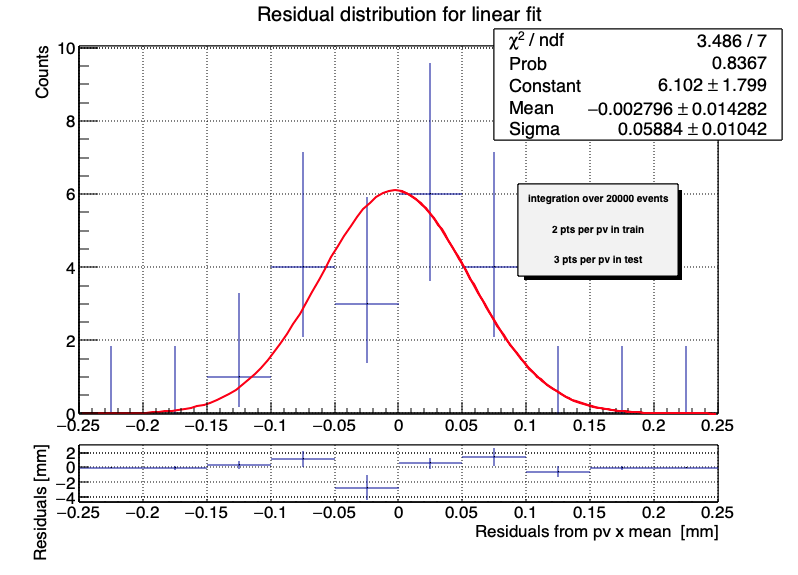
\includegraphics[width=\linewidth]{figures/x_res_veloC_MC.png}
    \caption{Residuals from the fit of the graph on the left. }\label{fig:x_veloC_res_MC}
    \end{subfigure}
    \caption{Linearity of the first PC divided by $\mu=5.5$ with respect to  virtual VELO C position shifts in x component, alongside the residuals distribution fitted with a Gaussian distribution.}
    \label{fig:x_veloC_MC}
\end{figure}
\begin{figure}
    \centering
    \begin{subfigure}{0.48\textwidth}
    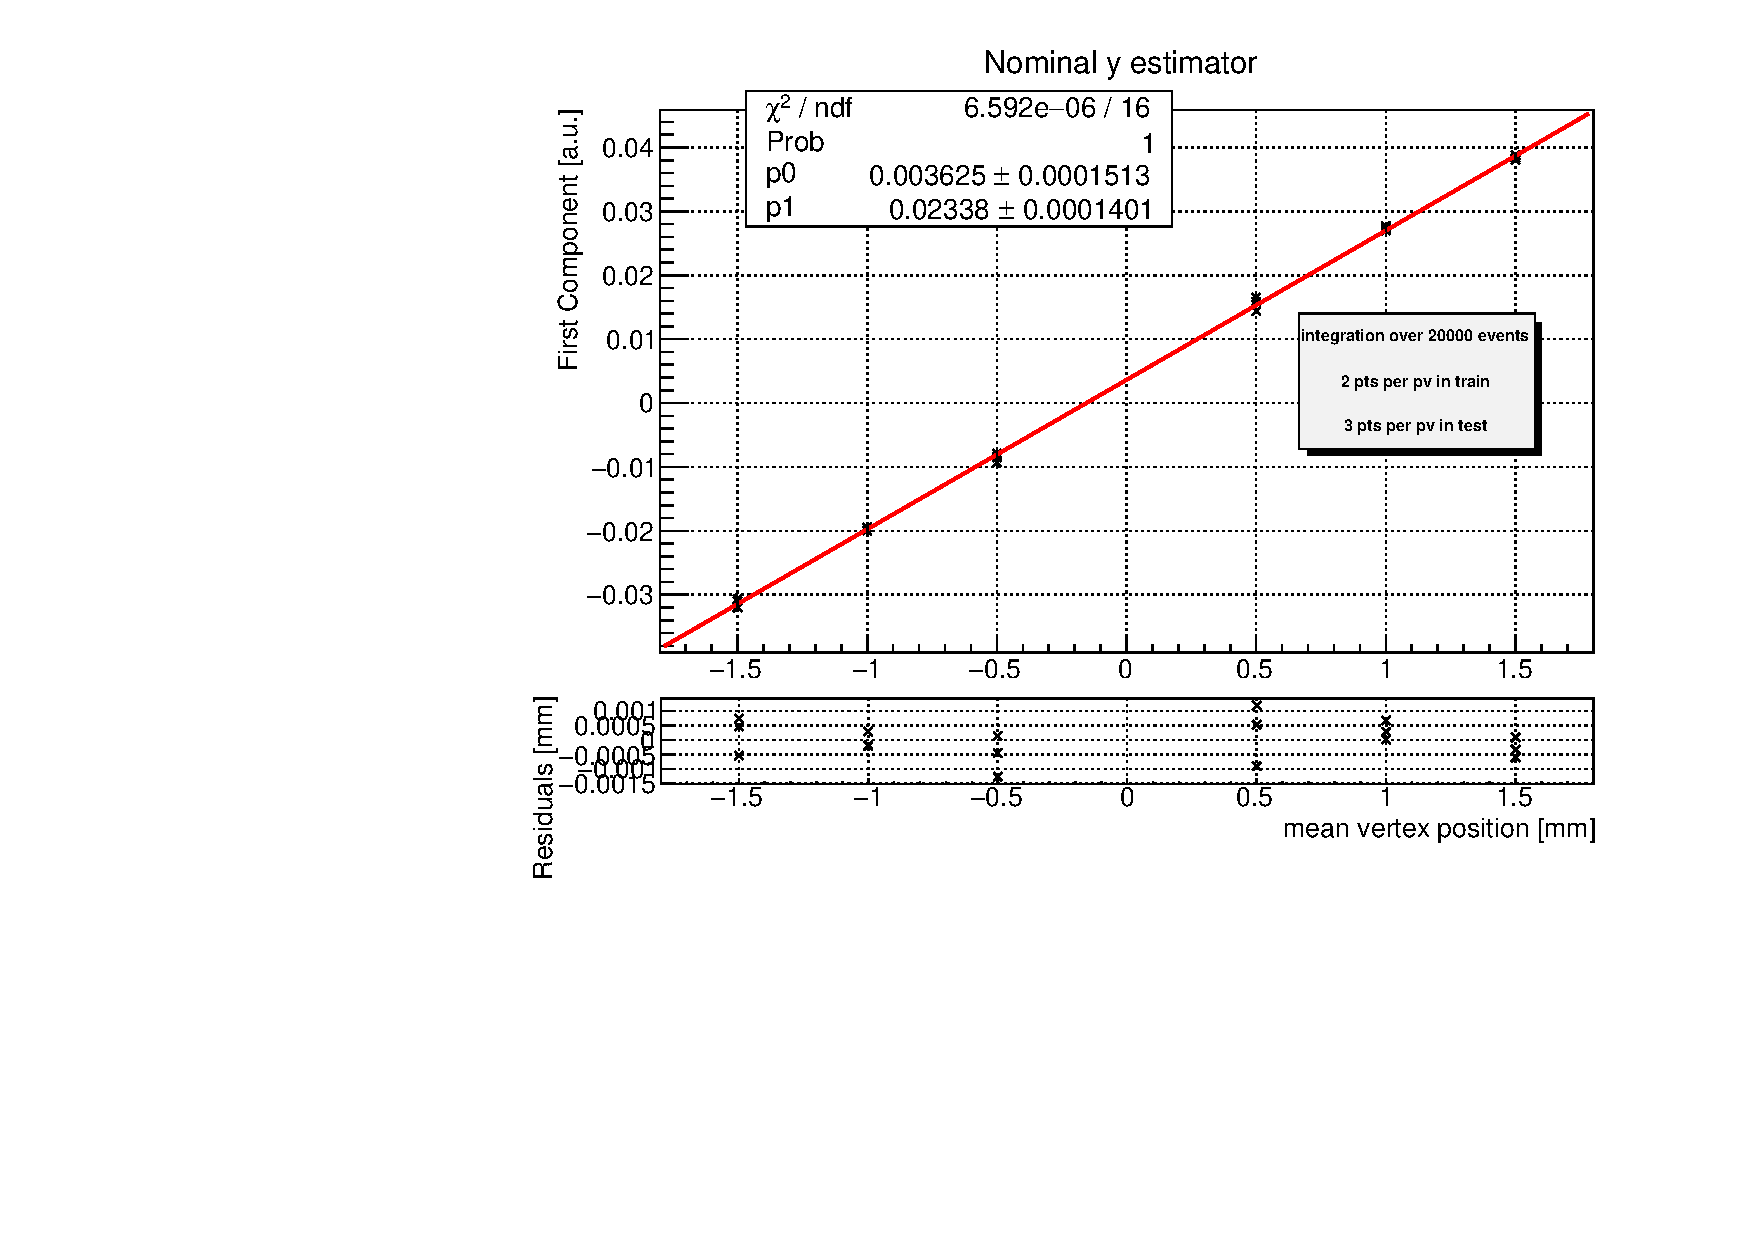
\includegraphics[width=\linewidth]{figures/y_fit_veloC_MC_normalised.pdf}
    \caption{Linear Fit}\label{fig:y_veloC_fit_MC}
    \end{subfigure}
    \begin{subfigure}{0.48\textwidth}
    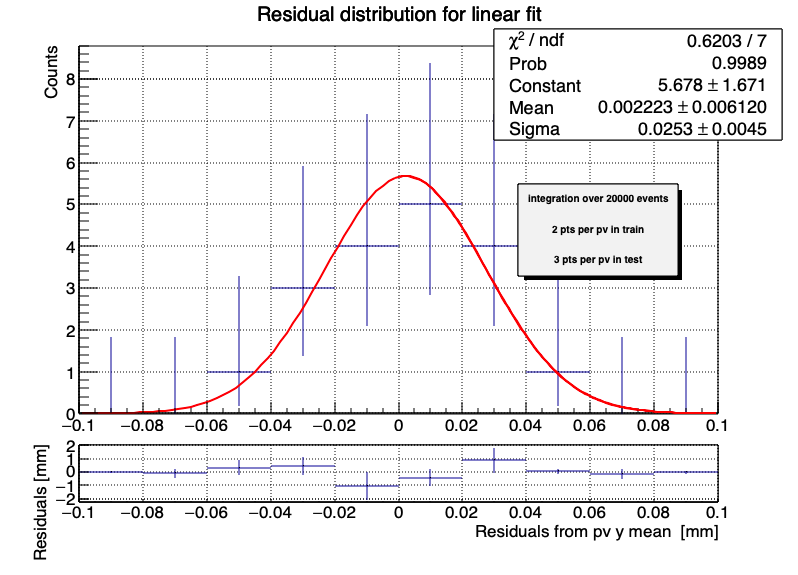
\includegraphics[width=\linewidth]{figures/y_res_veloC_MC.png}
    \caption{Residuals from the fit of the graph on the left. }\label{fig:y_veloC_res_MC}
    \end{subfigure}
    \caption{Linearity of the first PC divided by $\mu=5.5$ with respect to  virtual VELO C position shifts in y component, alongside the residuals distribution fitted with a Gaussian distribution.}
    \label{fig:y_veloC_MC}
\end{figure}

\begin{figure}
    \centering
    \begin{subfigure}{0.48\textwidth}
    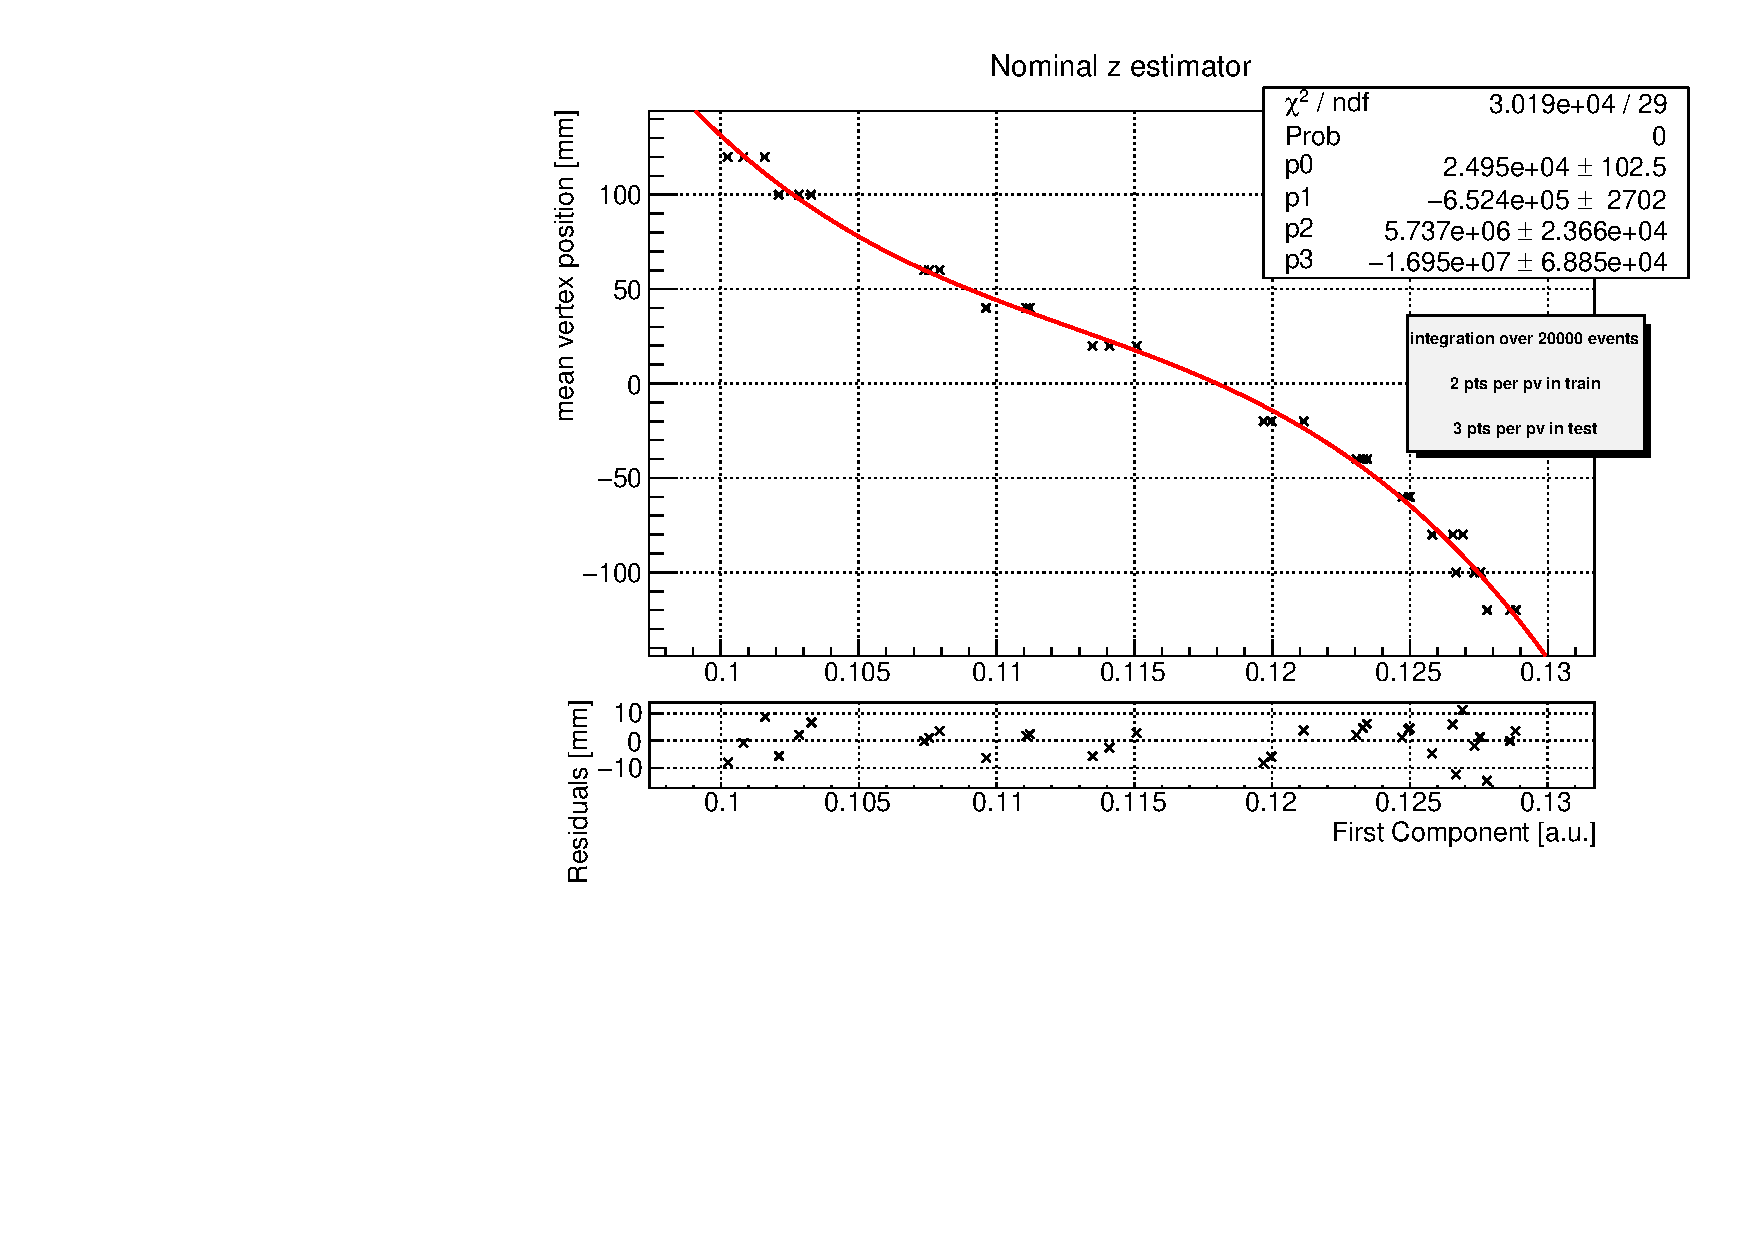
\includegraphics[width=\linewidth]{figures/z_fit_veloC_MC_residuals.pdf}
    \caption{Cubic Fit}\label{fig:z_veloC_fit_MC}
    \end{subfigure}
    \begin{subfigure}{0.48\textwidth}
    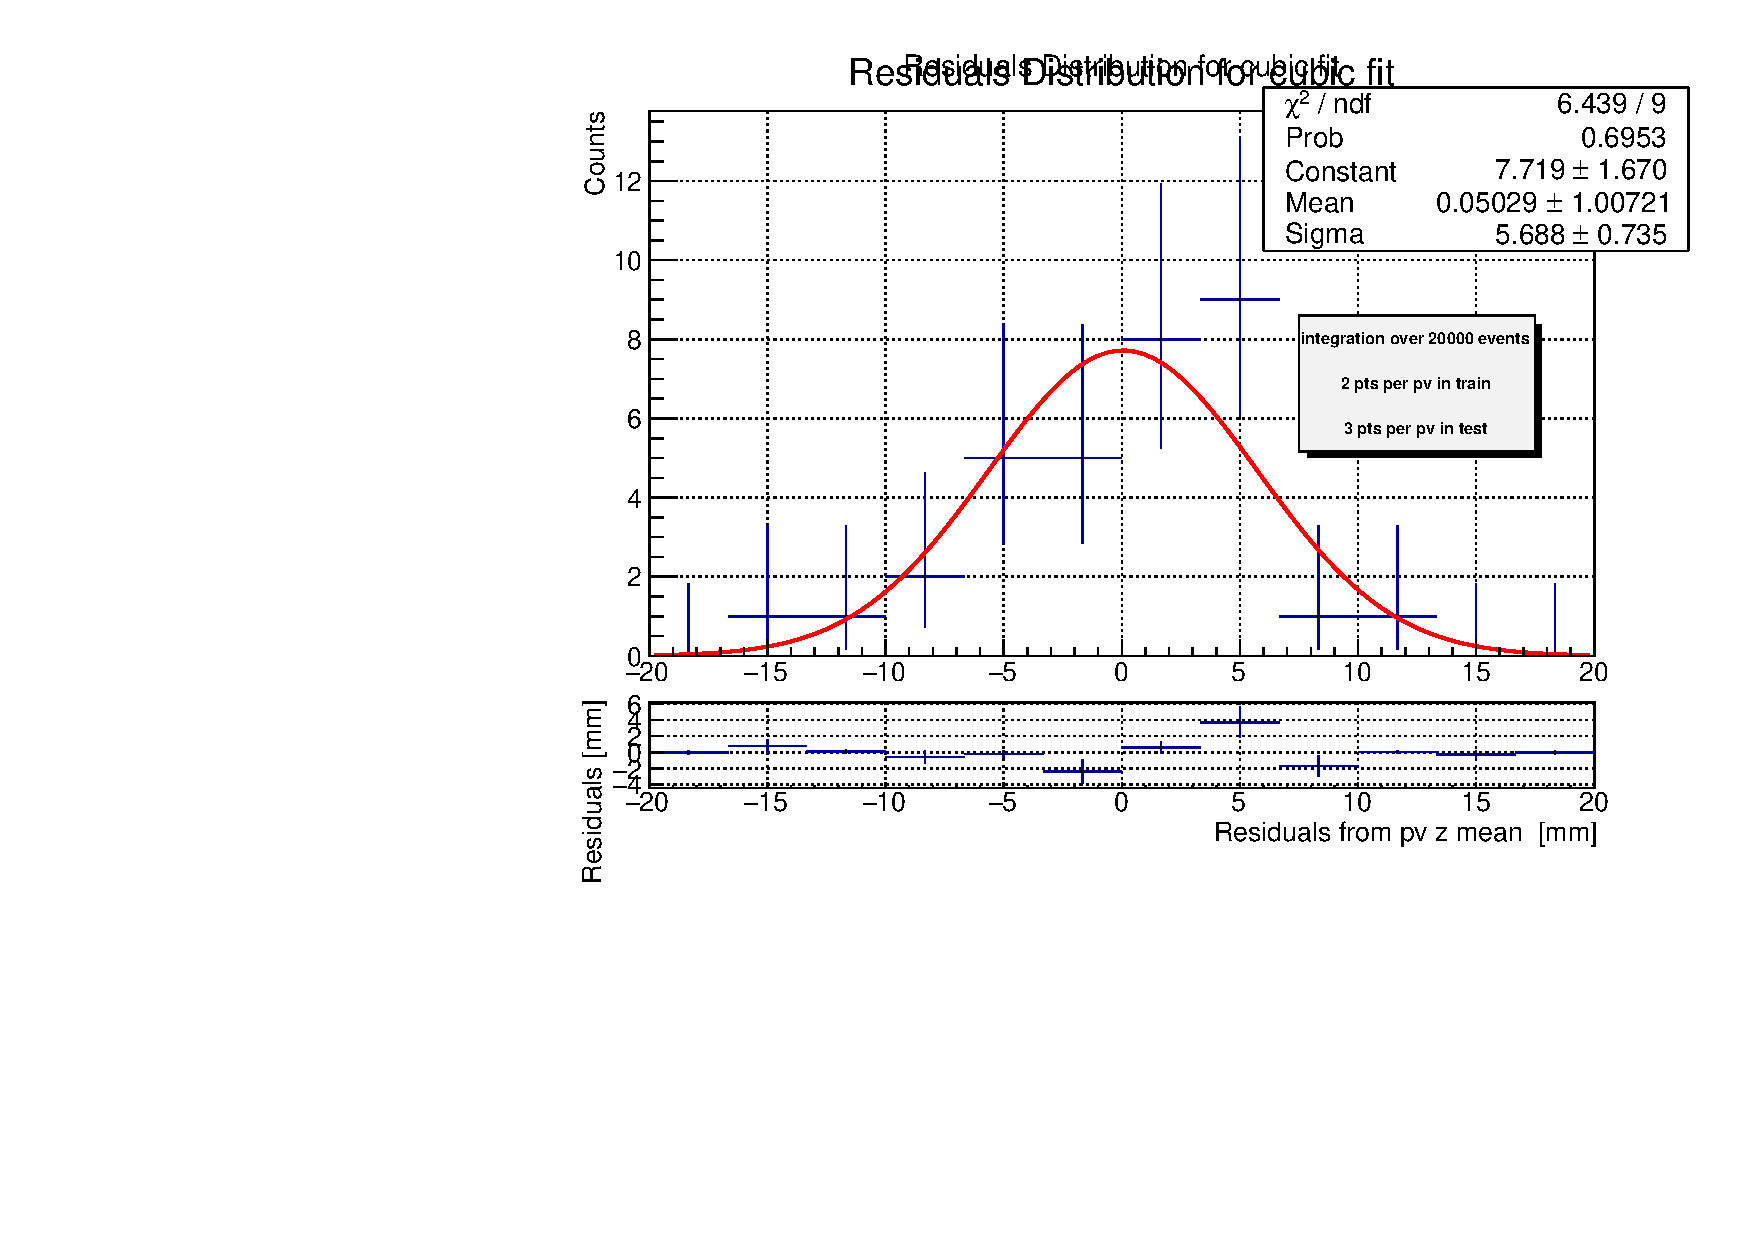
\includegraphics[width=\linewidth]{figures/z_res_veloC_MC_normalised.pdf}
    \caption{Residuals from the fit of the graph on the left. }\label{fig:z_veloC_res_MC}
    \end{subfigure}
    \caption{Cubic relationship between the first PC divided by $\mu=5.5$ with respect to virtual VELO C position shifts in the z component, alongside the residuals distribution fitted with a Gaussian distribution.}
    \label{fig:z_veloC_MC}
\end{figure}

As one can see, for both halves there is still a linear relationship between the scores and the virtual VELO positions in the $x$ and $y$ component, while the relationship remain cubic for the $z$ scores.  Furthermore, the Sigma estimated from the Gaussian fitted in the residuals histogram of Figures \ref{fig:x_veloA_res_MC}, \ref{fig:y_veloA_res_MC}, \ref{fig:z_veloA_res_MC}, \ref{fig:x_veloC_res_MC}, \ref{fig:y_veloC_res_MC}, \ref{fig:z_veloC_res_MC} show that the resolution is estimated to be between \SI{25}{\micro\meter} and \SI{81}{\micro\meter} for the transverse components $x$ and $y$, while for the $z$ component the value is around \SI{7}{\milli\meter}. As in the previous chapter, we expect the resolution for the $z$ component to be worse than the ones of the variables in the transverse plane to the beamline, since the luminous region is more spread along the $z$ direction, as explained in Section \ref{sec:MC}.

Since the relationship is essentially of the same form of equation \eqref{x_hat_corrected}, we can estimate the various coefficients from the fit performed in the scatter plots \ref{fig:x_veloA_fit_MC}, \ref{fig:y_veloA_fit_MC}, \ref{fig:z_veloA_fit_MC}, \ref{fig:x_veloC_fit_MC}, \ref{fig:y_veloC_fit_MC}, \ref{fig:z_veloC_fit_MC}. Regarding the $z$ variable, the coefficients are directly the ones plotted in the canvas. For the $x$ and $y$ components, we have to invert the relationship. In fact
\begin{equation}
    y = p1\cdot x +p0 \quad  \Longrightarrow \quad  x = \frac{y}{p1}-\frac{p0}{p1},
\end{equation}
meaning that the coefficients of equations \eqref{x_hat_corrected} need to be computed as 
\begin{equation}
    a = \frac{1}{p1} \qquad b = -\frac{p0}{p1}.
\end{equation}
We can therefore write the estimator for each side $s$=A,C using \eqref{eq:velo_hat}, with the various coefficients reported in Table~\ref{tab:coefficients}.
\begin{equation}
\begin{split}
    \hat{x}^{s} &= a_x^s \frac{t^x_1}{\mu} + b_x^s\\%\qquad
    \hat{y}^{s} &=a_y^s \frac{t^y_1}{\mu} + b_y^s \\%\qquad
    \hat{z}^{s} &=a_z^s\biggl(\frac{t^z_1}{\mu}\biggr)^3 + b_z^s\biggl(\frac{t^z_1}{\mu}\biggr)^2 + c_z^s \frac{t^z_1}{\mu} + d^s
    \end{split} \label{eq:velo_hat}
    \end{equation}
    
\begin{table}
\centering
\begin{tabular}{c|c|c|c|c|c|c}
coefficient  & $x_A$   & $y_A$   & $z_A$      & $x_C$   & $y_C$  & $z_C$      \\\hline
a & $44.29$  & $-43.97$ &  $-23008090$    & $-43.05$ & $42.77$ &   $-16950459$   \\
b & $-11.63$ & $0.1272$ & $8408082$   & $11.99$  & $-0.15$ &  $5736989$ \\
c &        &        & $-103031$   &        &       &  $-652426 $  \\
d &        &        &  $42358$ &        &       & $24954$
\end{tabular}
\caption{Summary of the coefficients for each estimator in the form of equation \eqref{eq:velo_hat}}\label{tab:coefficients}
\end{table}

\section{Calibration on real data}
We can perform another calibration for the $x$ and $y$ estimators of both VELO halves by directly relying on real collision data, using once again the mini VdM performed on April 6th, 2024. 
Once again, we perform the exercise of of thinking the beamline as fixed in space and the VELO moving with respect to this reference. By doing so, we can use the same ramps that were used to calibrate the luminous region estimators in the previous chapter. For the comparison, we rely on the reconstructed position of the VELO halves provided by the monitoring tasks of the VELO system, that reads a subset of minimum bias events at \SI{30}{\mega\hertz}. 

\begin{figure}
    \centering
    \begin{subfigure}{0.48\textwidth}
    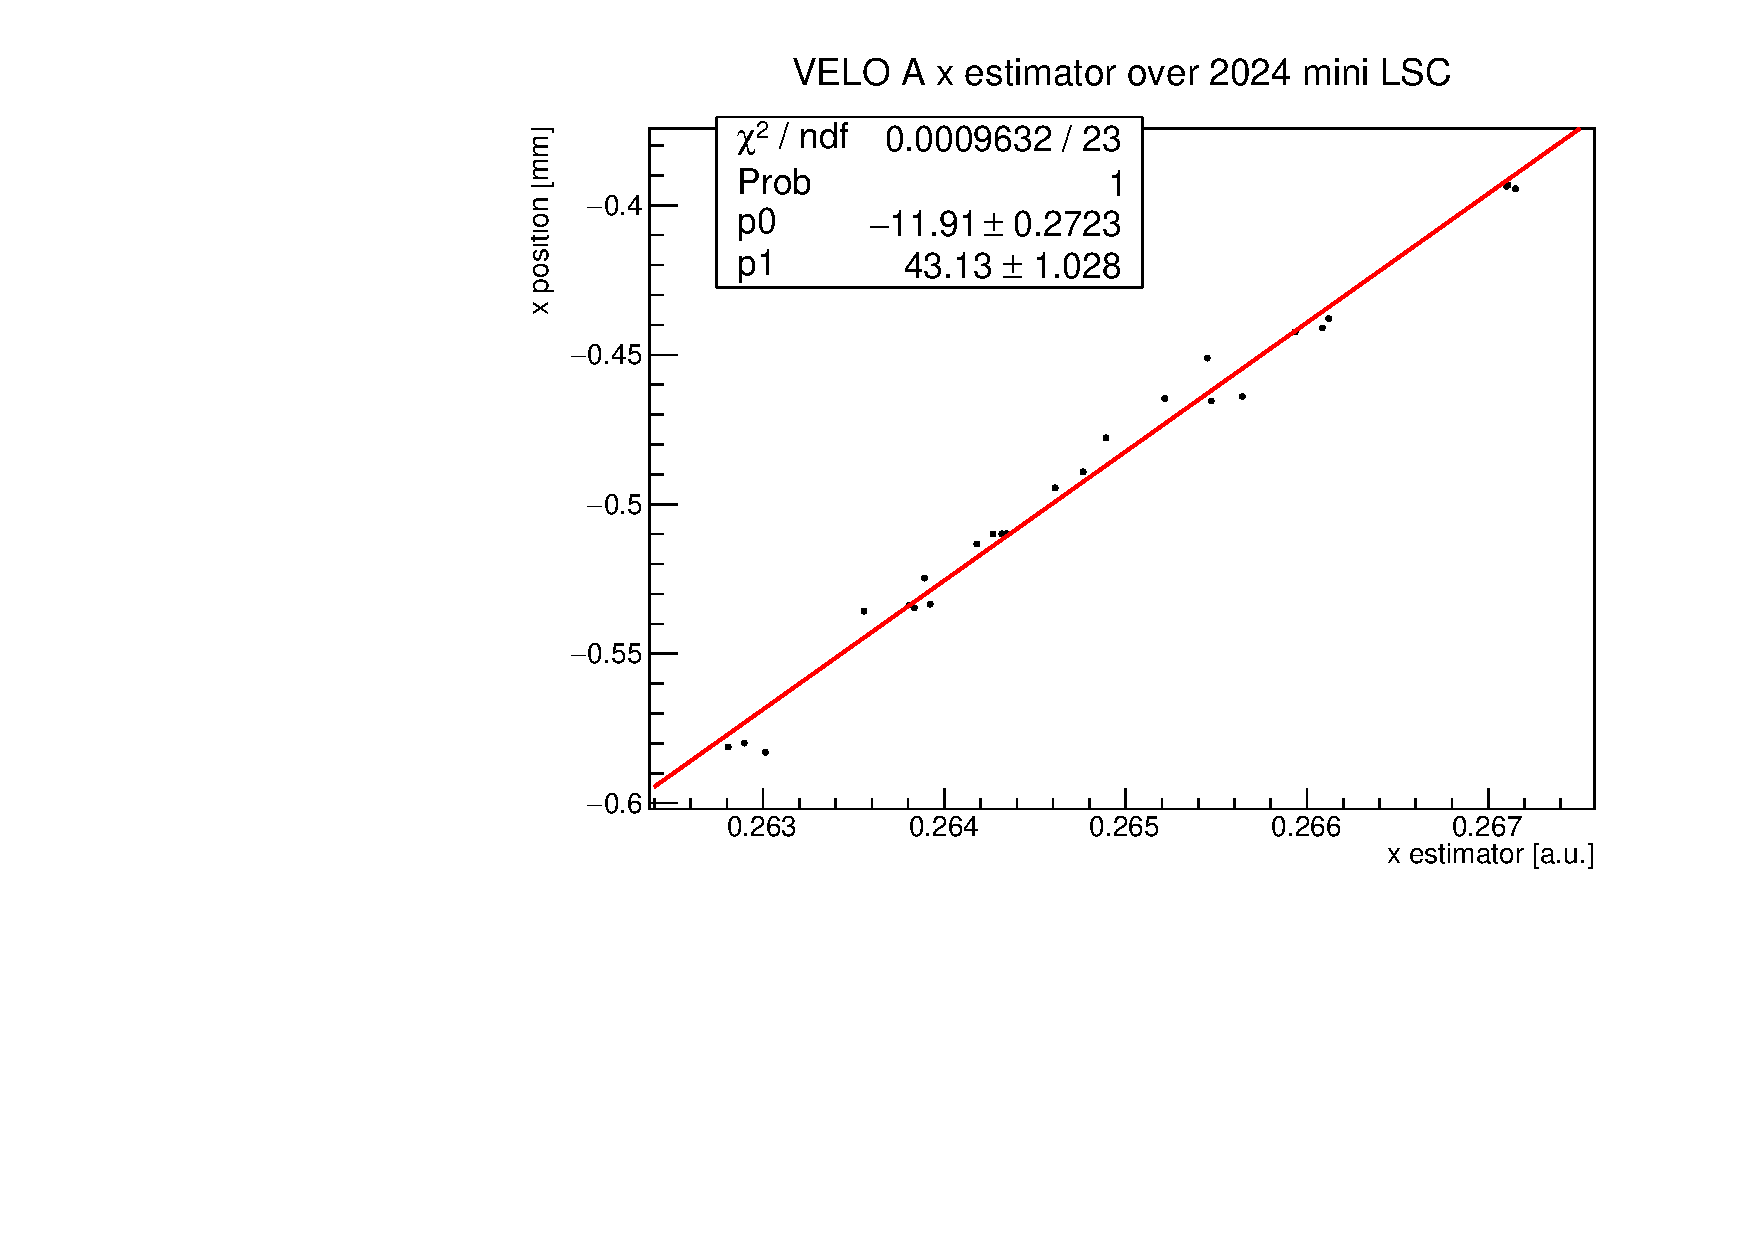
\includegraphics[width=\linewidth]{figures/x_fit_VELO_A_data.pdf}
    \caption{Linear Fit}\label{fig:x_veloA_fit_data}
    \end{subfigure}
    \begin{subfigure}{0.48\textwidth}
    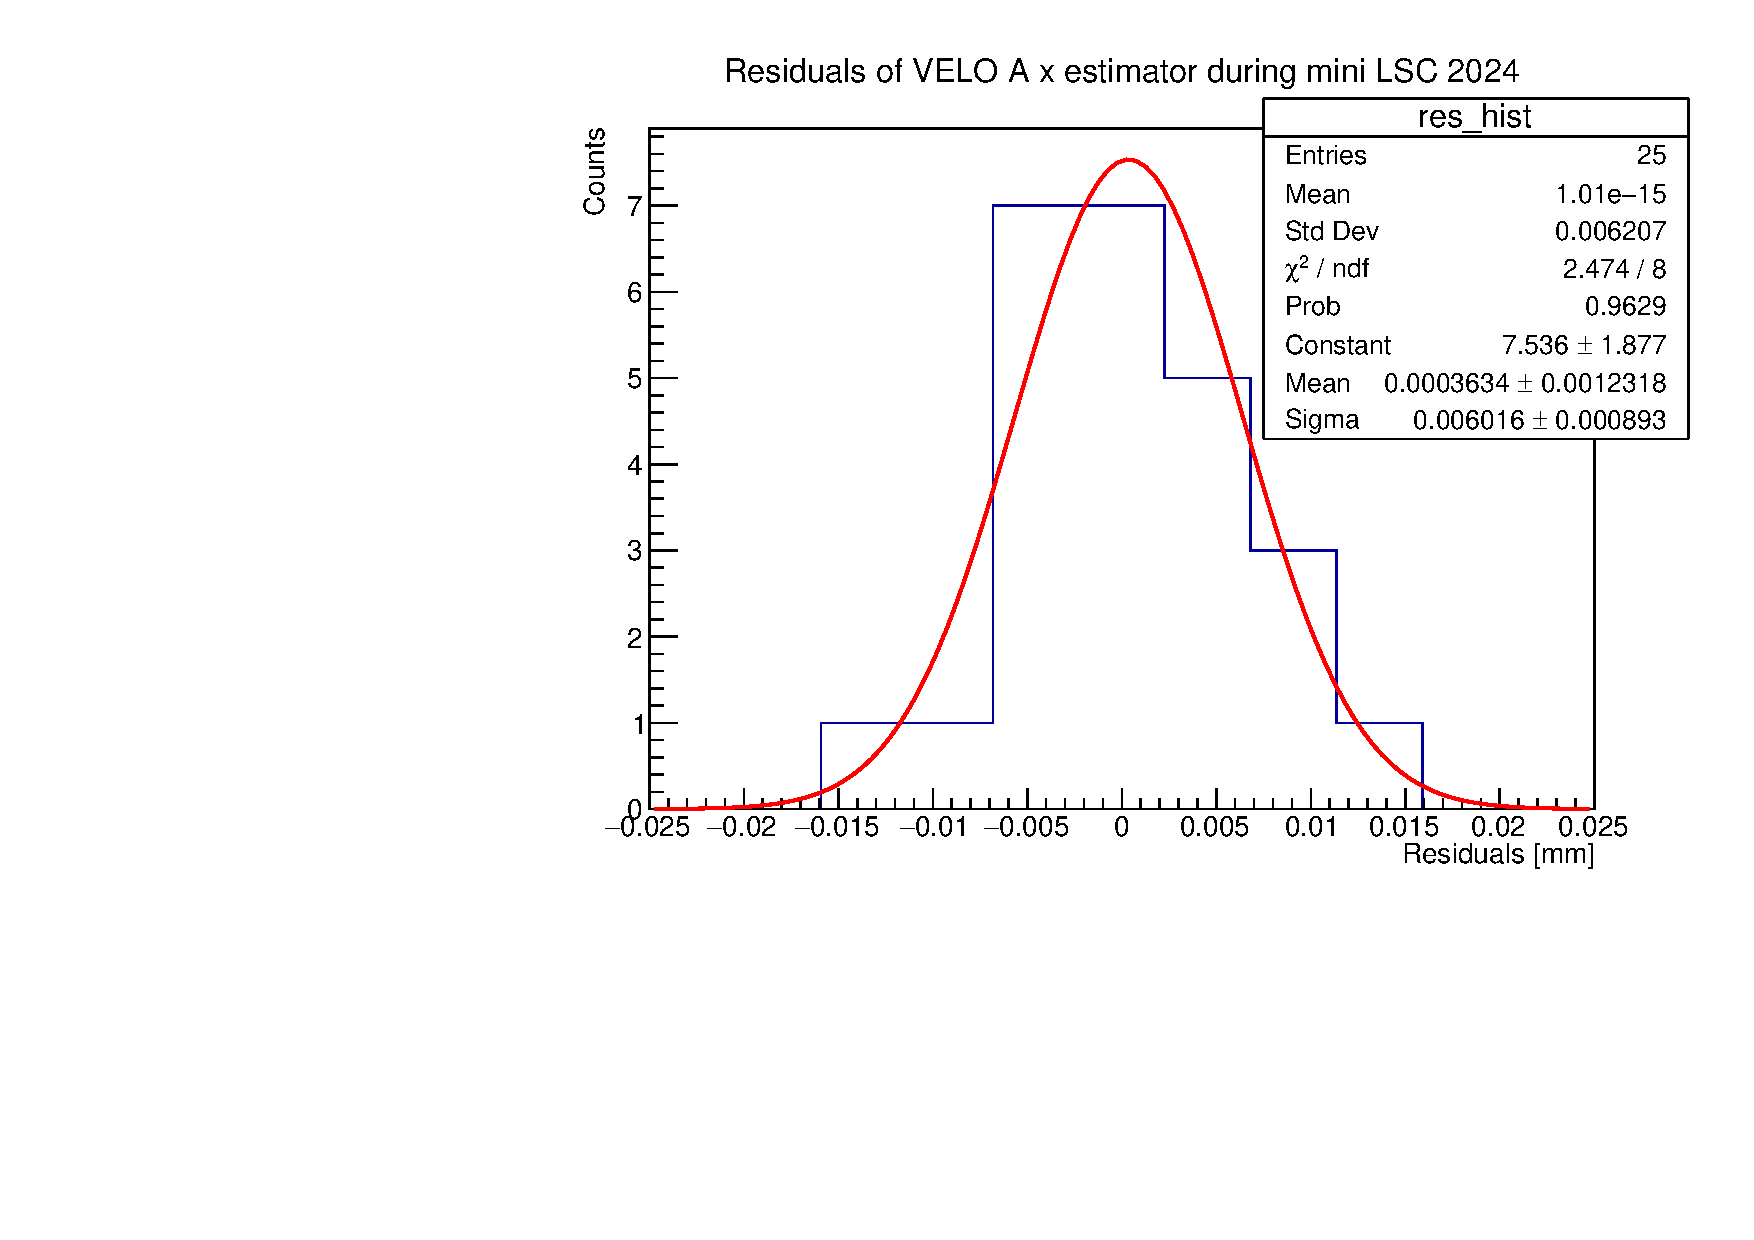
\includegraphics[width=\linewidth]{figures/x_res_VELO_A_data.pdf}
    \caption{Residuals from the fit of the graph on the left. }\label{fig:x_veloA_res_data}
    \end{subfigure}
    \caption{Linearity of the first component calculated with the PCA with respect to virtual VELO A position shifts in x component, alongside the residuals distribution fitted with a Gaussian distribution.}
    \label{fig:x_veloA_data}
\end{figure}


\begin{figure}
    \centering
    \begin{subfigure}{0.48\textwidth}
    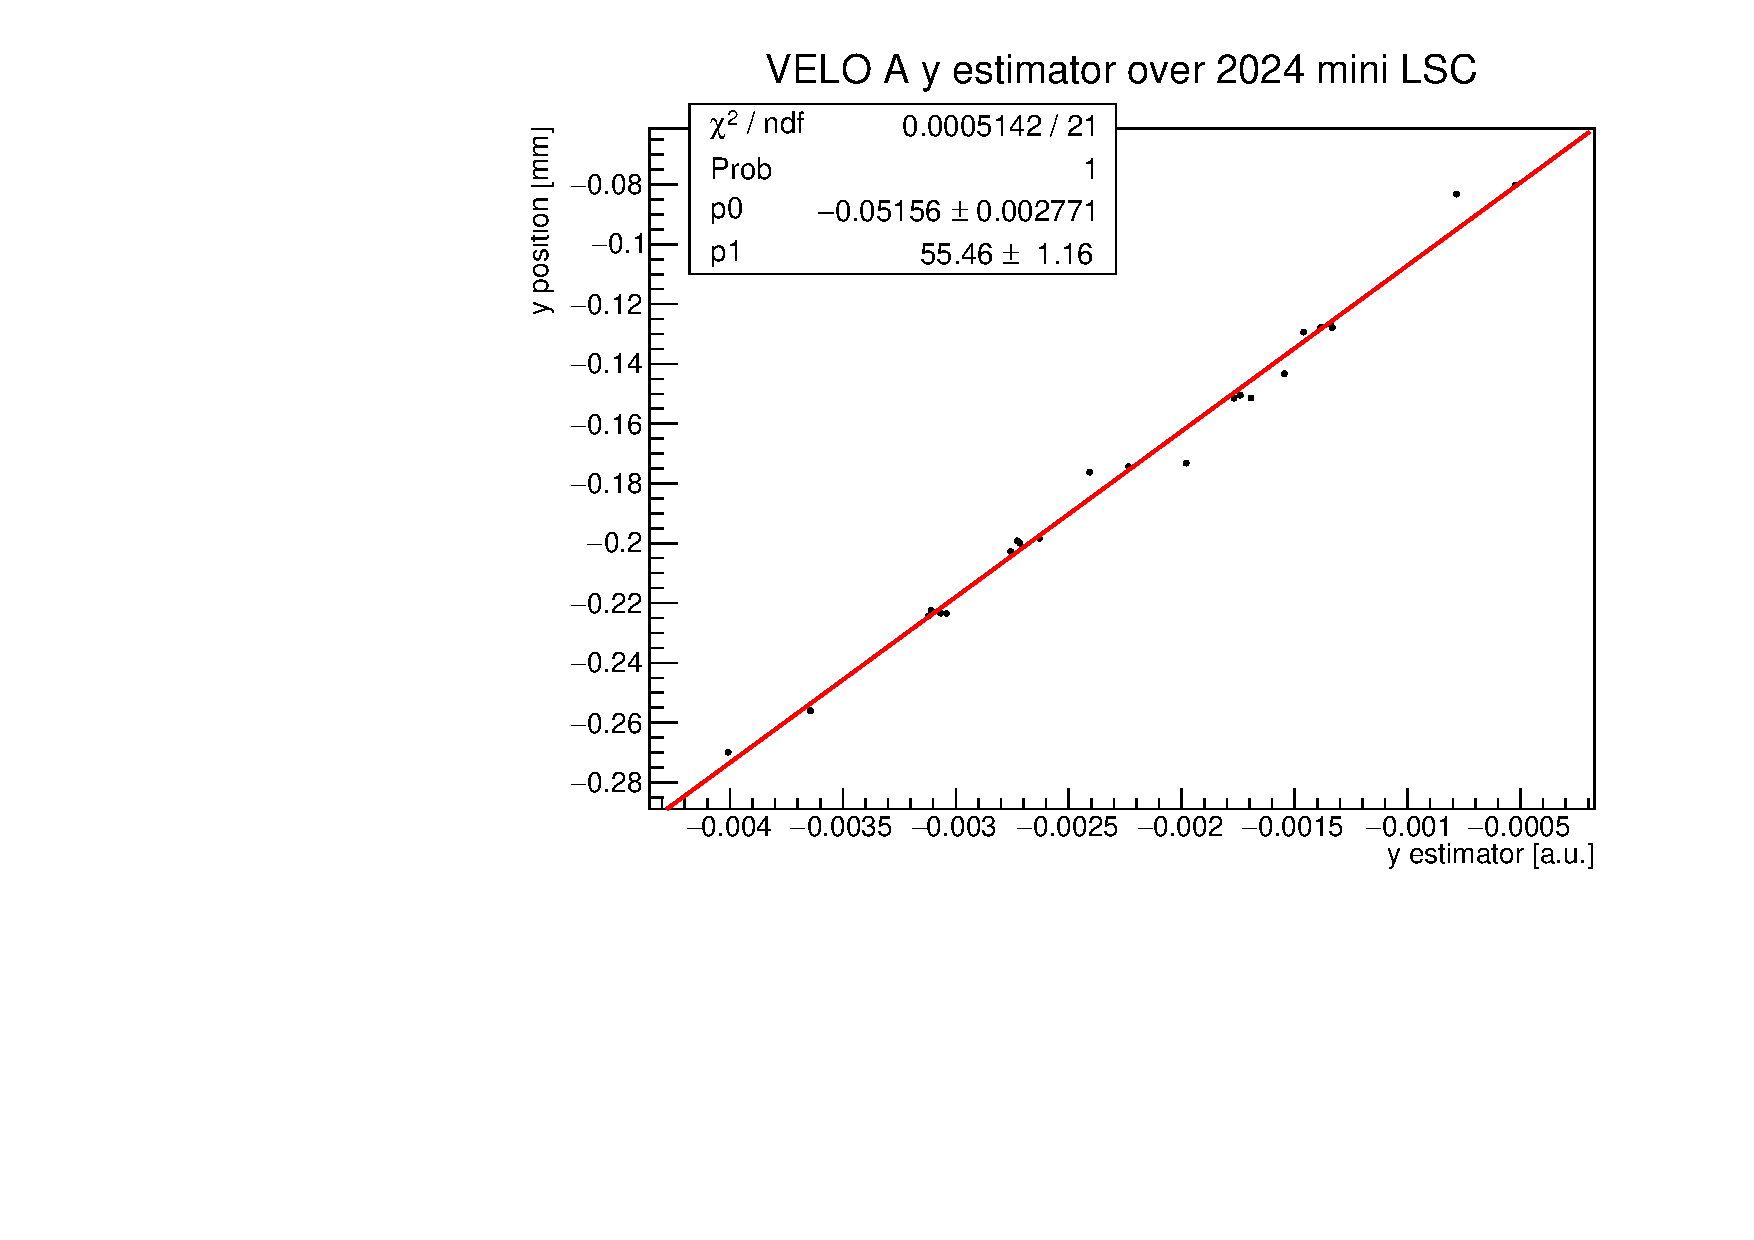
\includegraphics[width=\linewidth]{figures/y_fit_VELO_A_data.pdf}
    \caption{Linear Fit}\label{fig:y_veloA_fit_data}
    \end{subfigure}
    \begin{subfigure}{0.48\textwidth}
    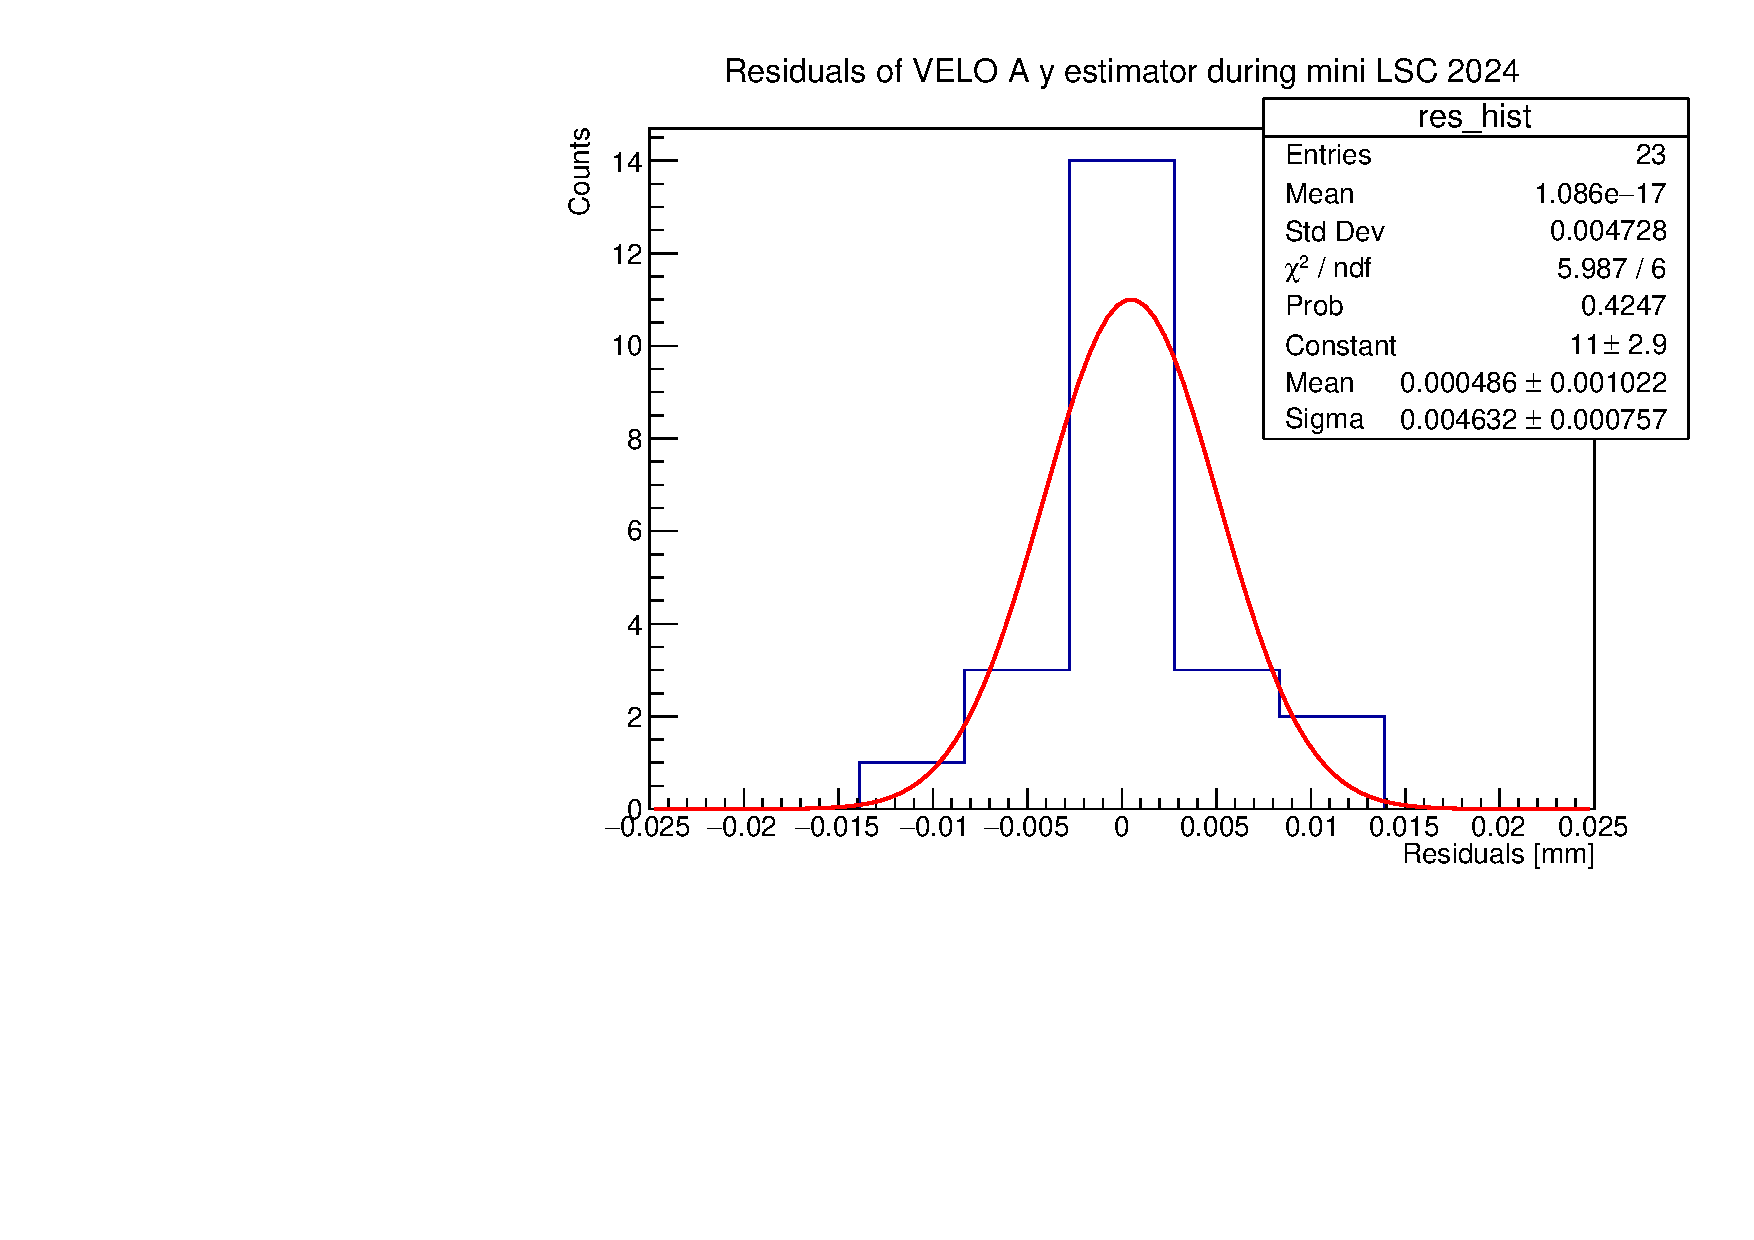
\includegraphics[width=\linewidth]{figures/y_res_VELO_A_data.pdf}
    \caption{Residuals from the fit of the graph on the left. }\label{fig:y_veloA_res_data}
    \end{subfigure}
    \caption{Linearity of the first component calculated with the PCA with respect to virtual VELO A position shifts in y component, alongside the residuals distribution fitted with a Gaussian distribution.}
    \label{fig:y_veloA_data}
\end{figure}



\begin{figure}
    \centering
    \begin{subfigure}{0.48\textwidth}
    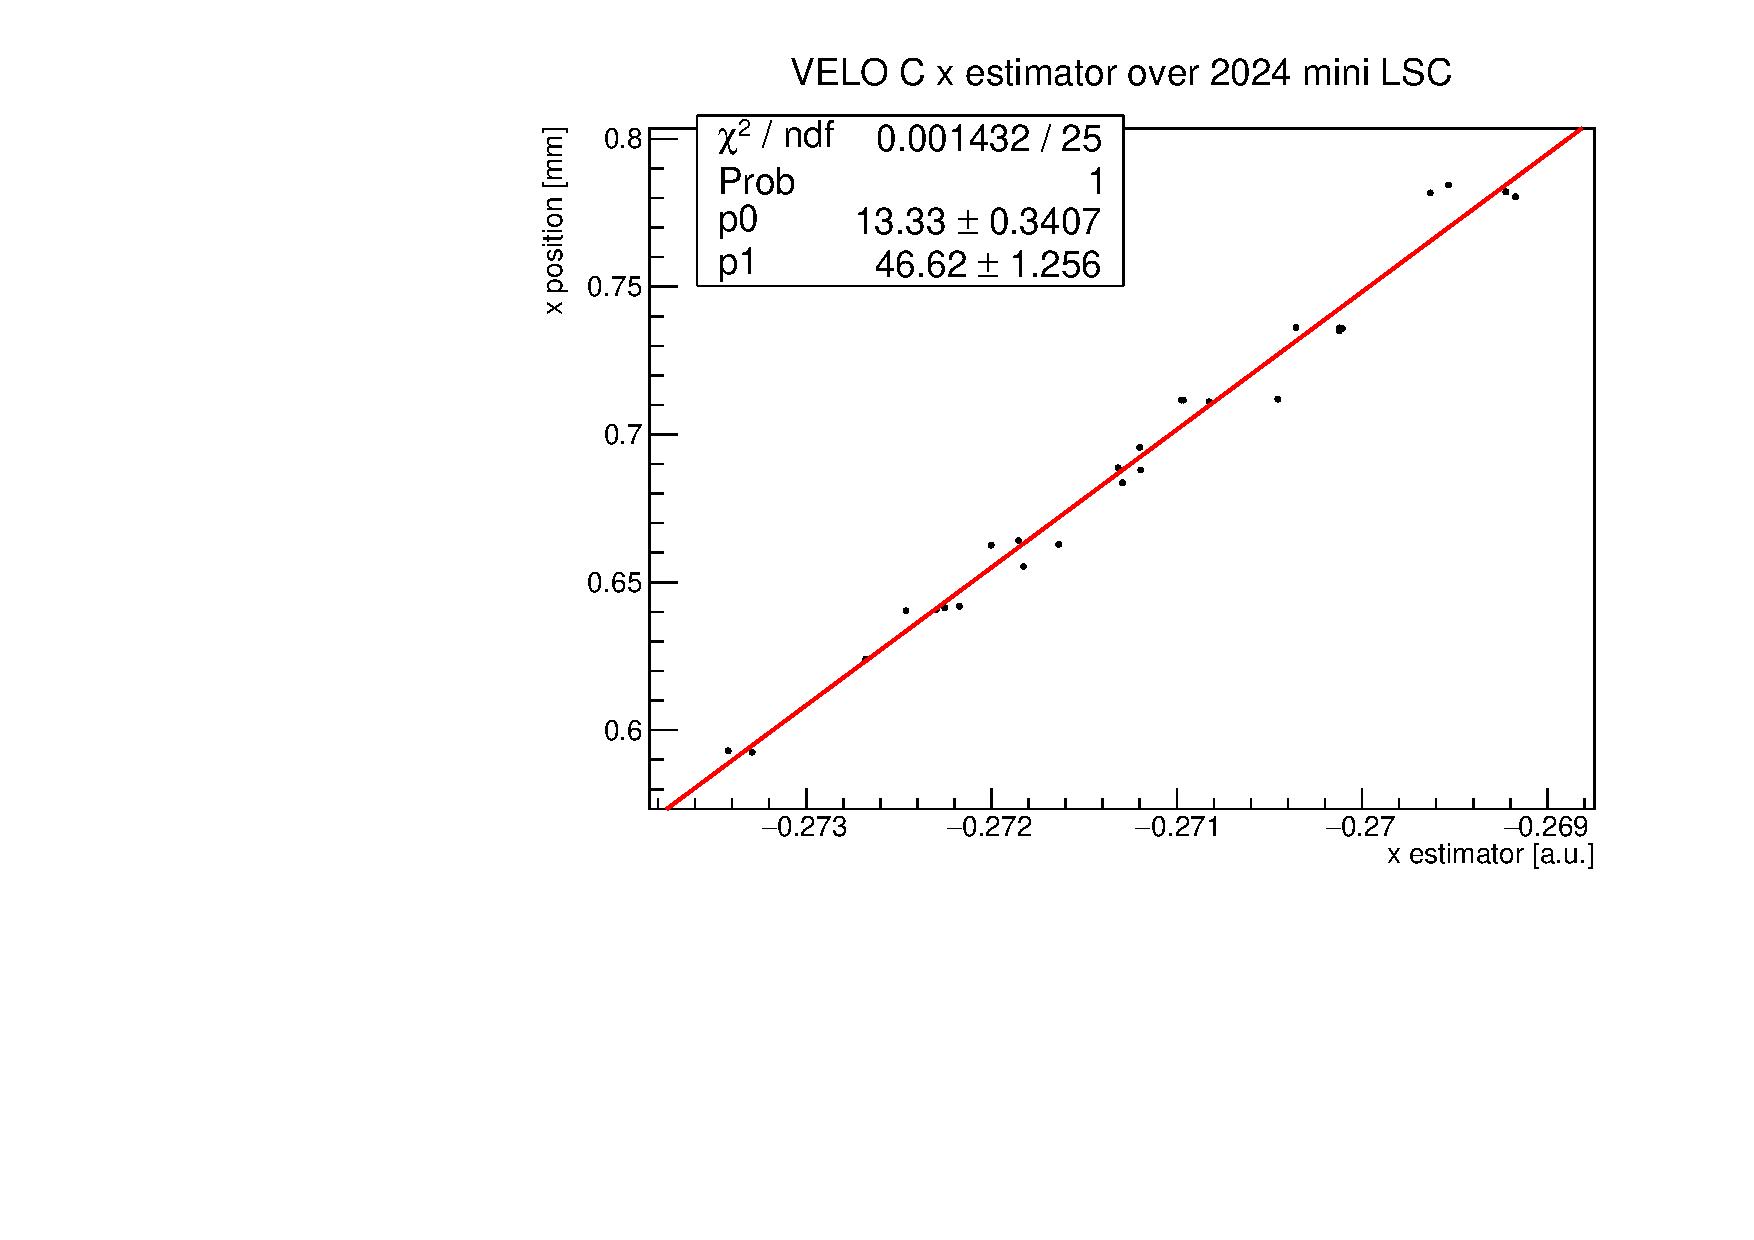
\includegraphics[width=\linewidth]{figures/x_fit_VELO_C_data.pdf}
    \caption{Linear Fit}\label{fig:x_veloC_fit_data}
    \end{subfigure}
    \begin{subfigure}{0.48\textwidth}
    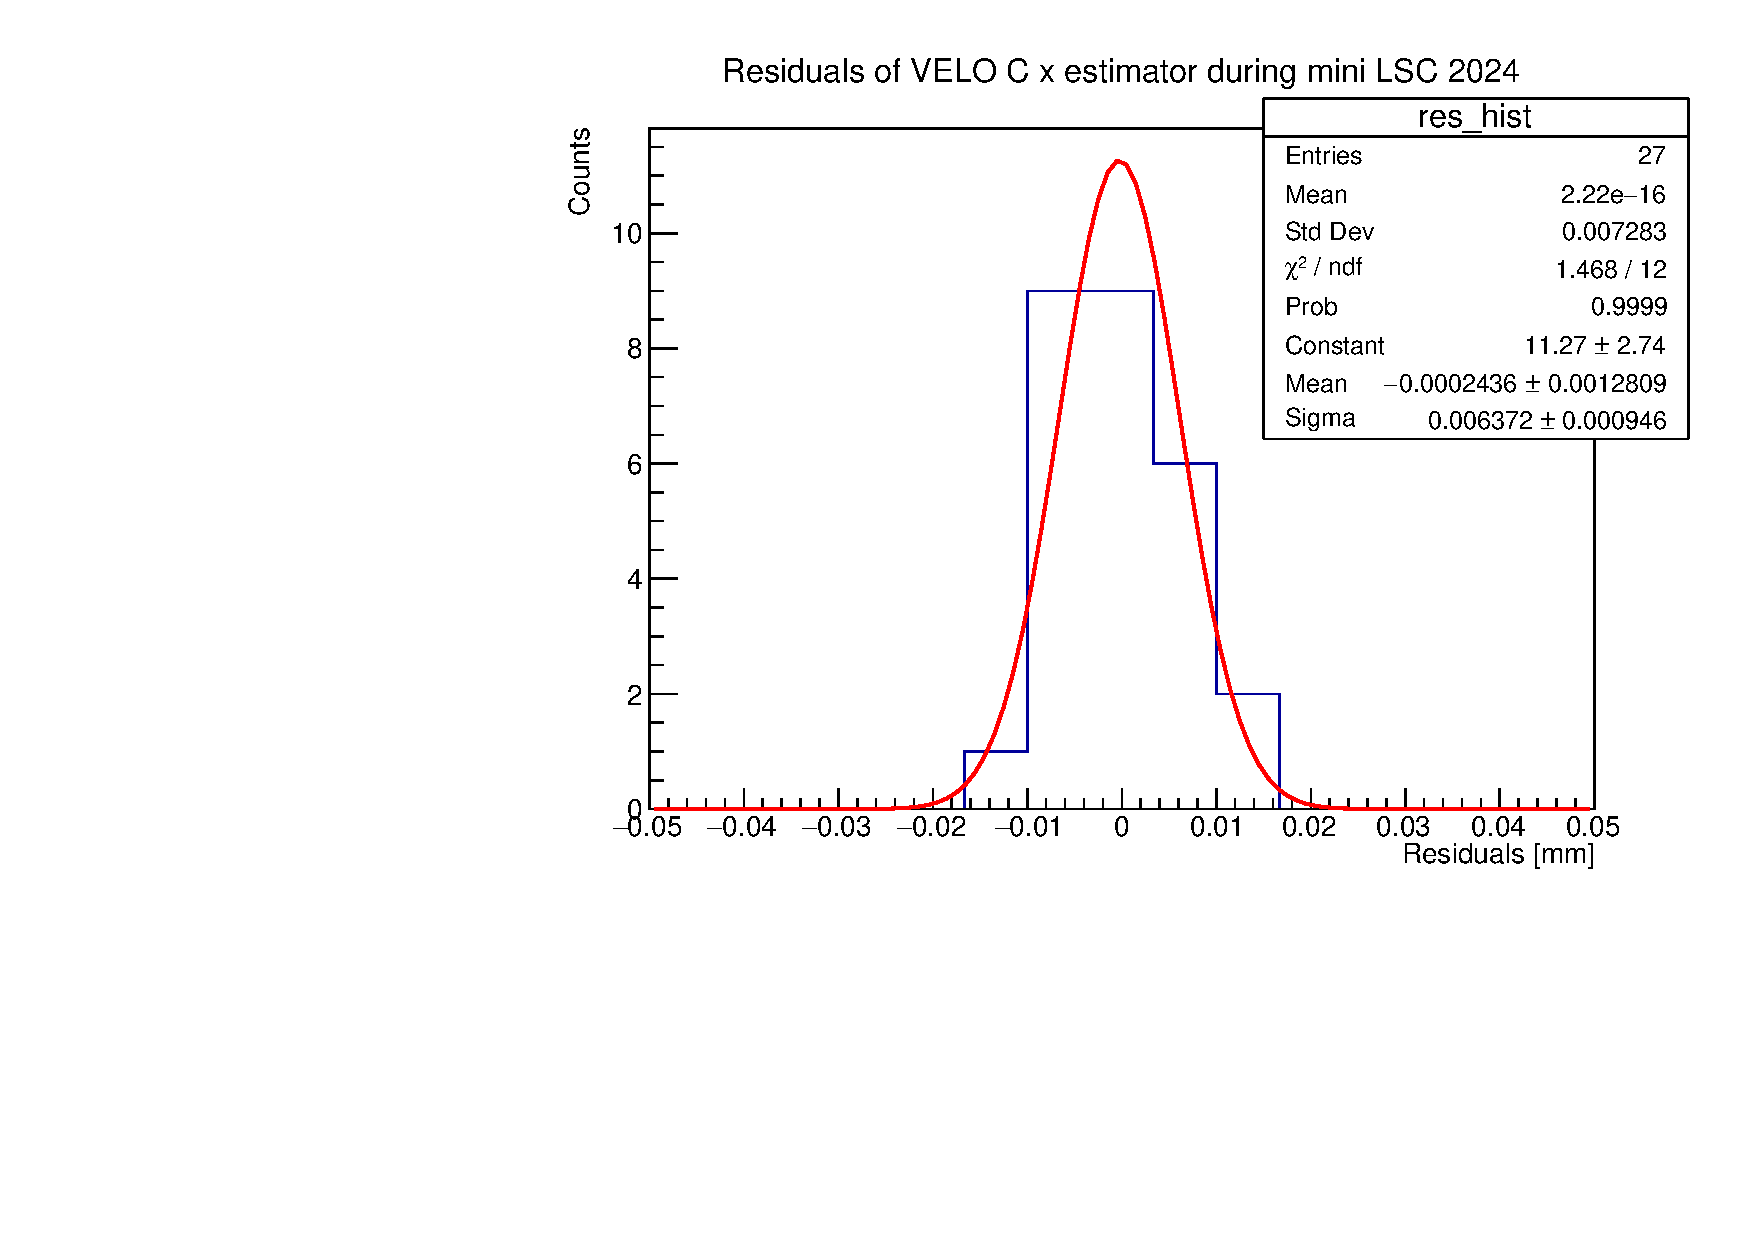
\includegraphics[width=\linewidth]{figures/x_res_VELO_C_data.pdf}
    \caption{Residuals from the fit of the graph on the left. }\label{fig:x_veloC_res_data}
    \end{subfigure}
    \caption{Linearity of the first component calculated with the PCA with respect to  virtual VELO C position shifts in x component, alongside the residuals distribution fitted with a Gaussian distribution.}
    \label{fig:x_veloC_data}
\end{figure}
\begin{figure}
    \centering
    \begin{subfigure}{0.48\textwidth}
    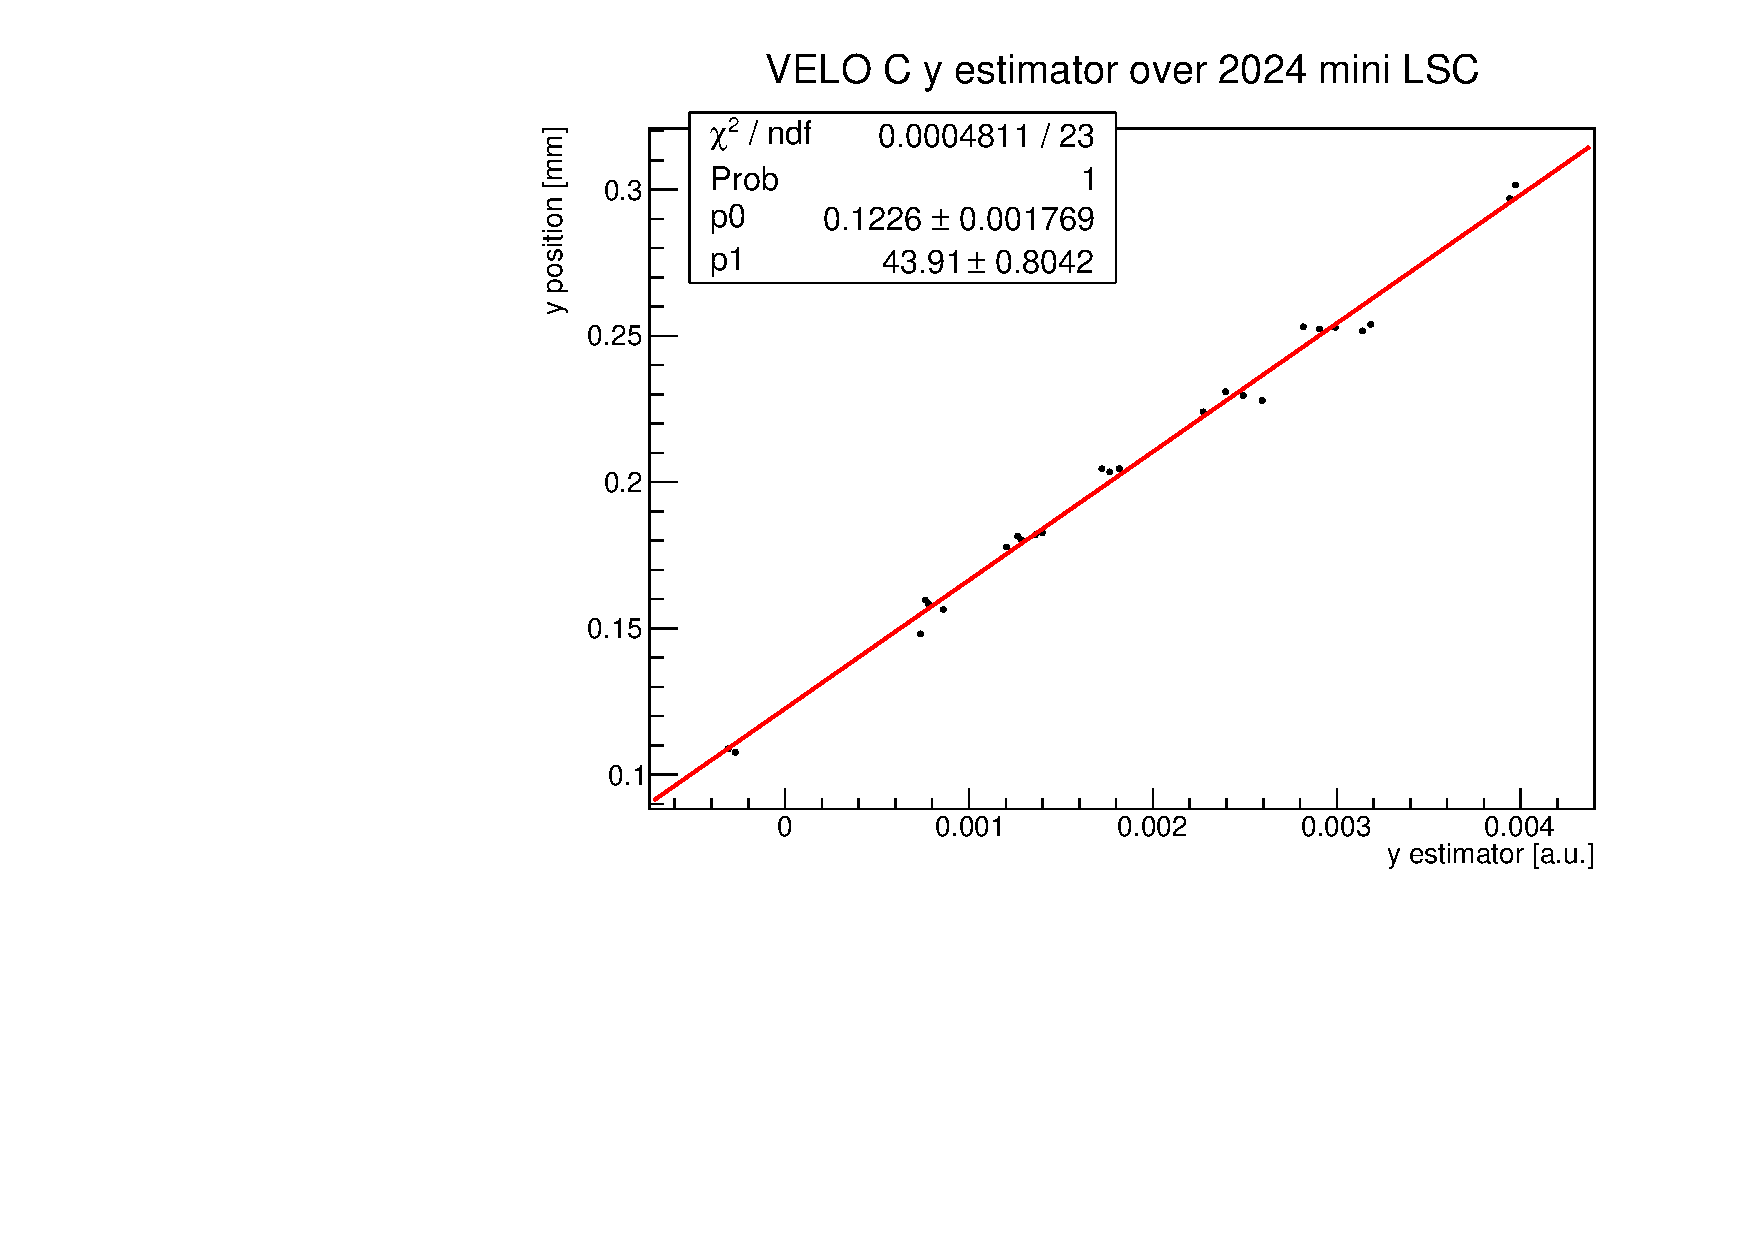
\includegraphics[width=\linewidth]{figures/y_fit_VELO_C_data.pdf}
    \caption{Linear Fit}\label{fig:y_veloC_fit_data}
    \end{subfigure}
    \begin{subfigure}{0.48\textwidth}
    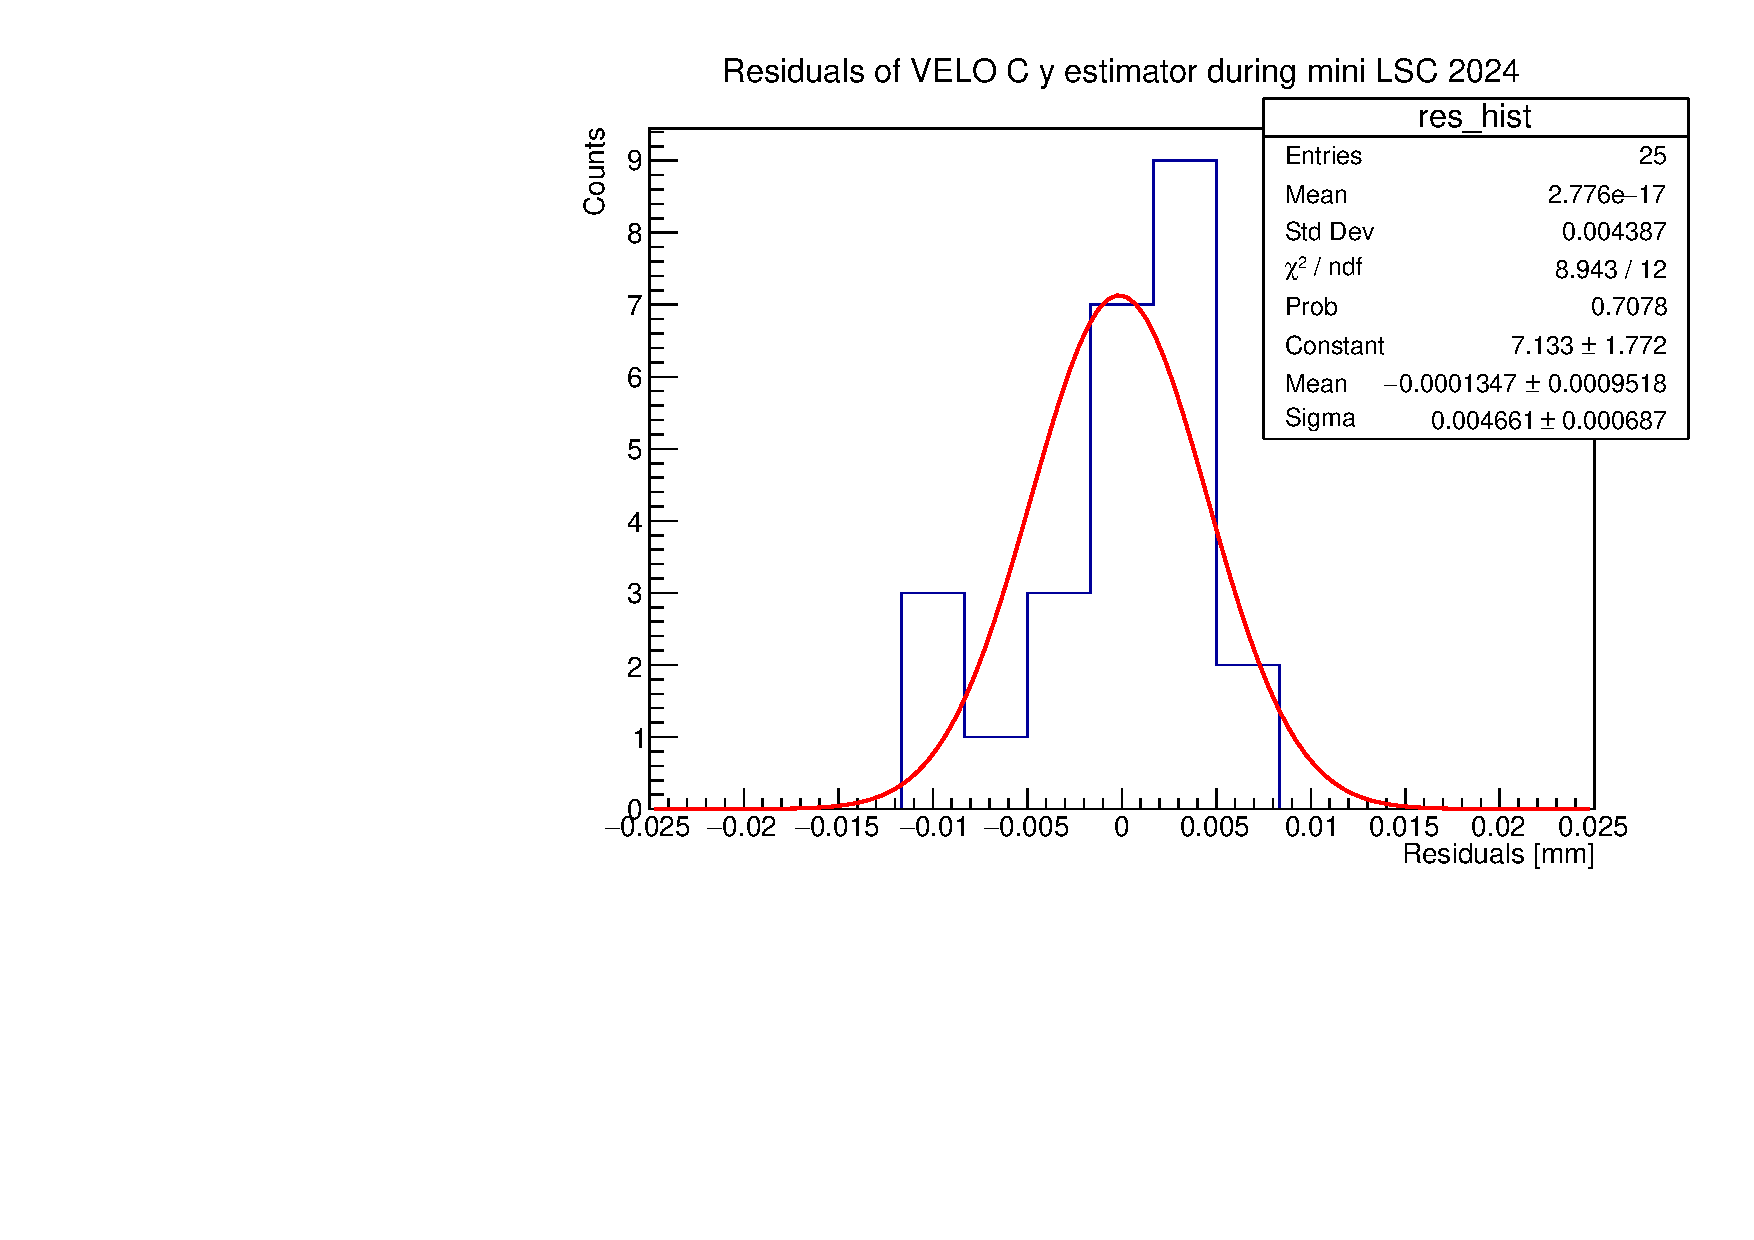
\includegraphics[width=\linewidth]{figures/y_res_VELO_C_data.pdf}
    \caption{Residuals from the fit of the graph on the left. }\label{fig:y_veloC_res_data}
    \end{subfigure}
    \caption{Linearity of the first component calculated with the PCA with respect to  virtual VELO C position shifts in y component, alongside the residuals distribution fitted with a Gaussian distribution.}
    \label{fig:y_veloC_data}
\end{figure}

The scatter plots alongside the residuals of the linear fitted function are reported in the Figures \ref{fig:x_veloA_data}, \ref{fig:y_veloA_data}, \ref{fig:x_veloC_data}, \ref{fig:y_veloC_data}, respectively for $\hat{x}_A$, $\hat{y}_A$, $\hat{x}_C$, $\hat{y}_C$. As we can see from these scatter plot the relationship is linear, and from these fitted line we can infer other parameters that allows to calculate the estimators $\hat{x}_A$, $\hat{y}_A$, $\hat{x}_C$, $\hat{y}_C$. In order to deal with the problem of outliers and missing counters, we apply the same algorithm \ref{alg:beamline} described at the end of Chapter \ref{chap:beamline}. 

We can see a preliminary result of this calibration in Figure \ref{fig:traceplot_xy}, where we report the traceplot of the estimators (blue and green) during a the two LSC compared with the position of the VELO halves estimated by the monitoring task (orange and red). The points used for the calibration are the ones of the first ramps in $x$ and $y$, meaning that starting from 13:32 ca the calibration holds and estimators estimate the quantity it should. This behaviour is appreciated particularly during the second ramp that starts in the $x$ component around 13:47.

\begin{figure}
    \centering
    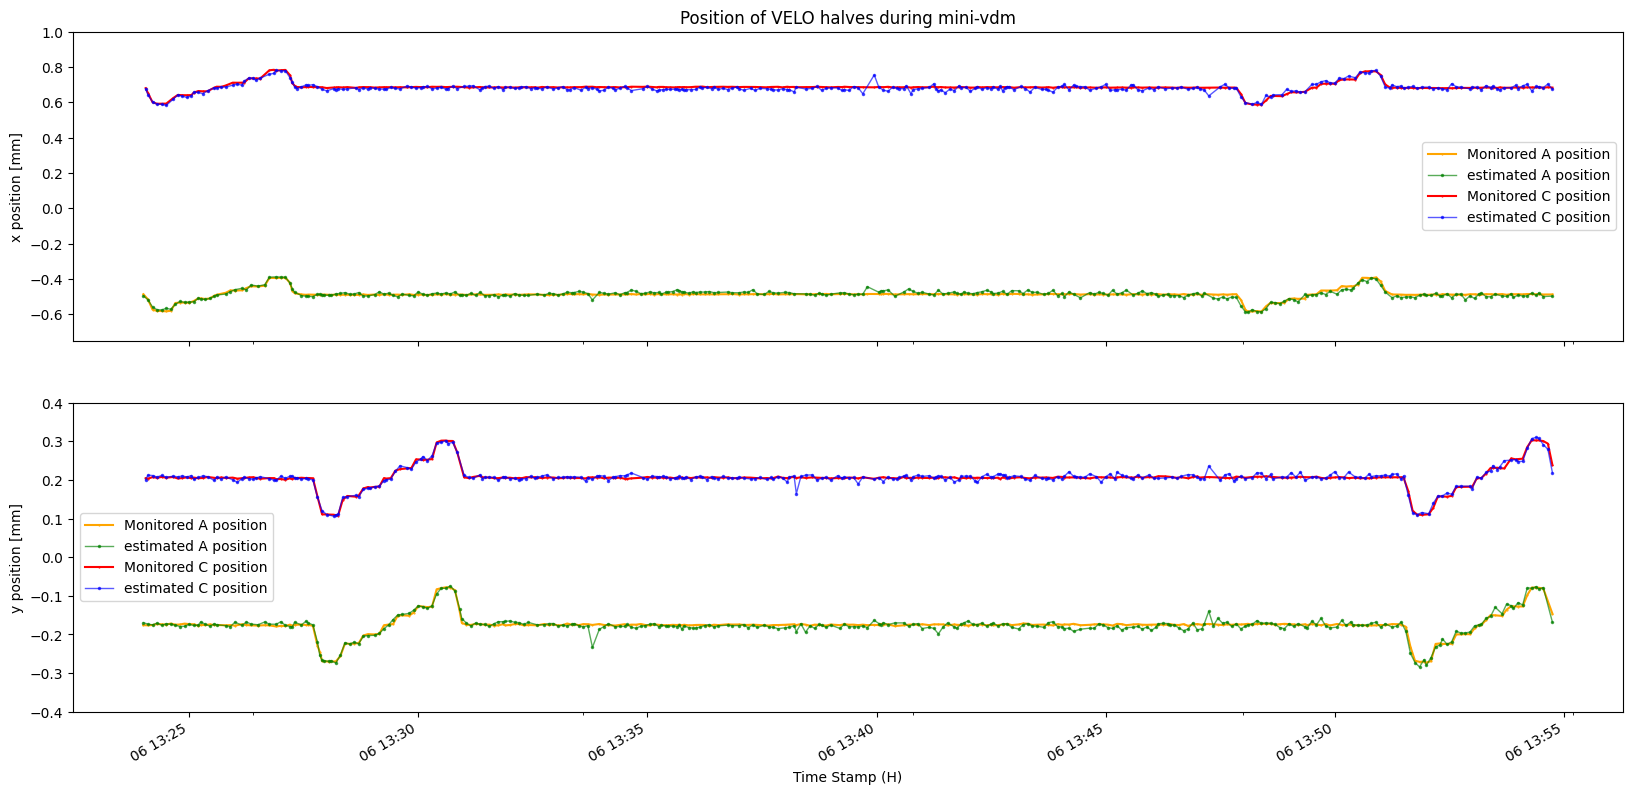
\includegraphics[width=\textwidth]{figures/traceplot_xy.png}
    \caption{Traceplot of the VELO position estimators across the two VdM scans. In the upper panel, the $x$ position is displayed. The red and orange lines correspond to the monitored position of the two VELO halves, while the blue and the green ones to the estimated position presented in this chapter. An analogue situation is displayed in the second panel, in the $y$ component.}
    \label{fig:traceplot_xy}
\end{figure}

A more quantitative analysis of the correctness of the estimated positions $\hat{x}_A$, $\hat{y}_{A}$, $\hat{x}_C$, $\hat{y}_C$ can be performed by producing a scatter plot between the estimated positions vs the relative reconstructed positions by the monitoring tasks of the VELO during the whole LSC fill. These scatter plot are available in Figures \ref{fig:xAfit_comparison}, \ref{fig:yAfit_comparison}, \ref{fig:xCfit_comparison}, \ref{fig:yCfit_comparison}, where on the left graph we performed a linear fit, while on the right we performed a Gaussian fit of the residuals. If there is total accordance between these to quantities we expected the angular coefficients to be $p1=1$ and the offset $p0=0$ of the fitted line. 
The results of these fit are summarised in Table \ref{tab:summary}. There is great accordance between the coefficients, since they all differ less than 2.1 $\sigma$ from their expected value $p1=1$ and $p0=0$. 


\begin{figure}
    \centering
    \begin{subfigure}{0.48\textwidth}
    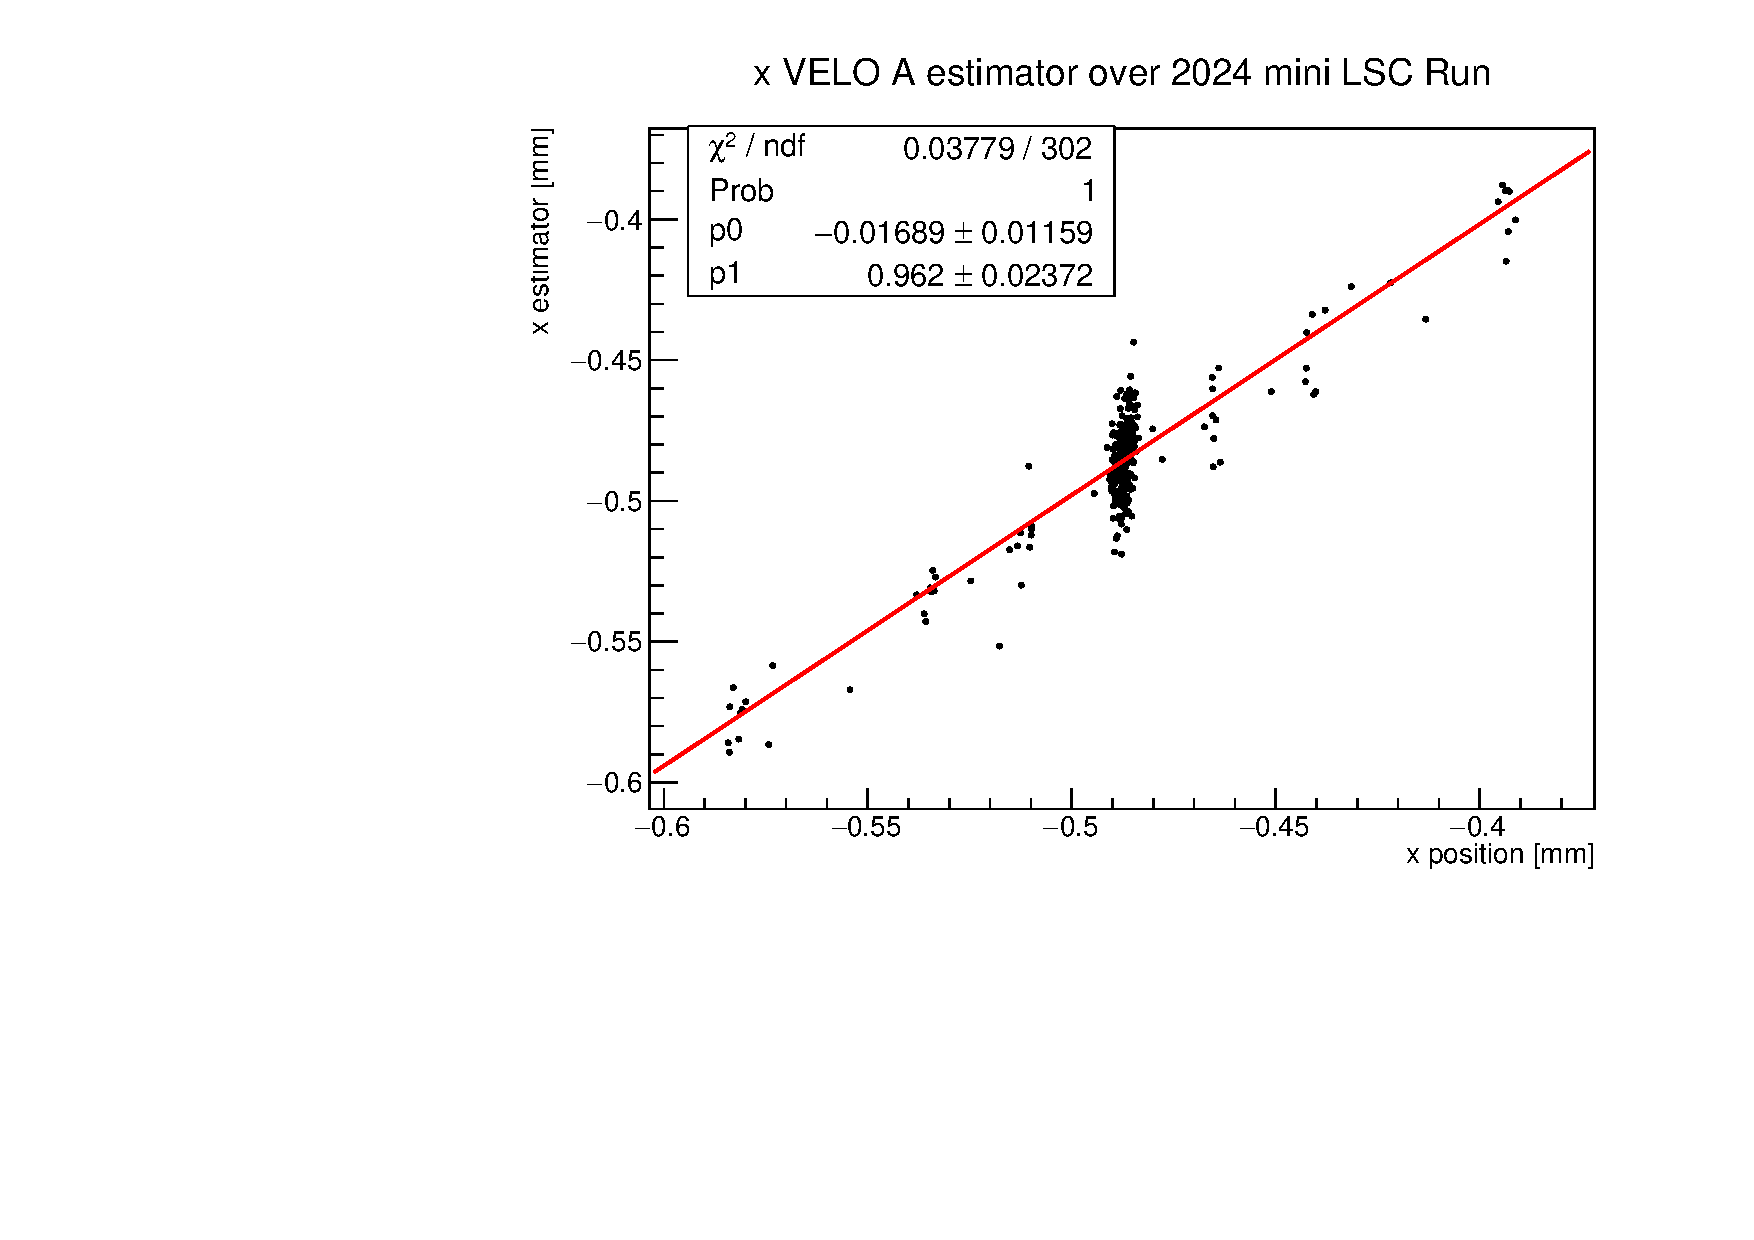
\includegraphics[width=\linewidth]{figures/xVeloA_fit_comparison.pdf}
    \caption{Linear Fit}\label{fig:xAfit_comparison}
    \end{subfigure}
    \begin{subfigure}{0.48\textwidth}
    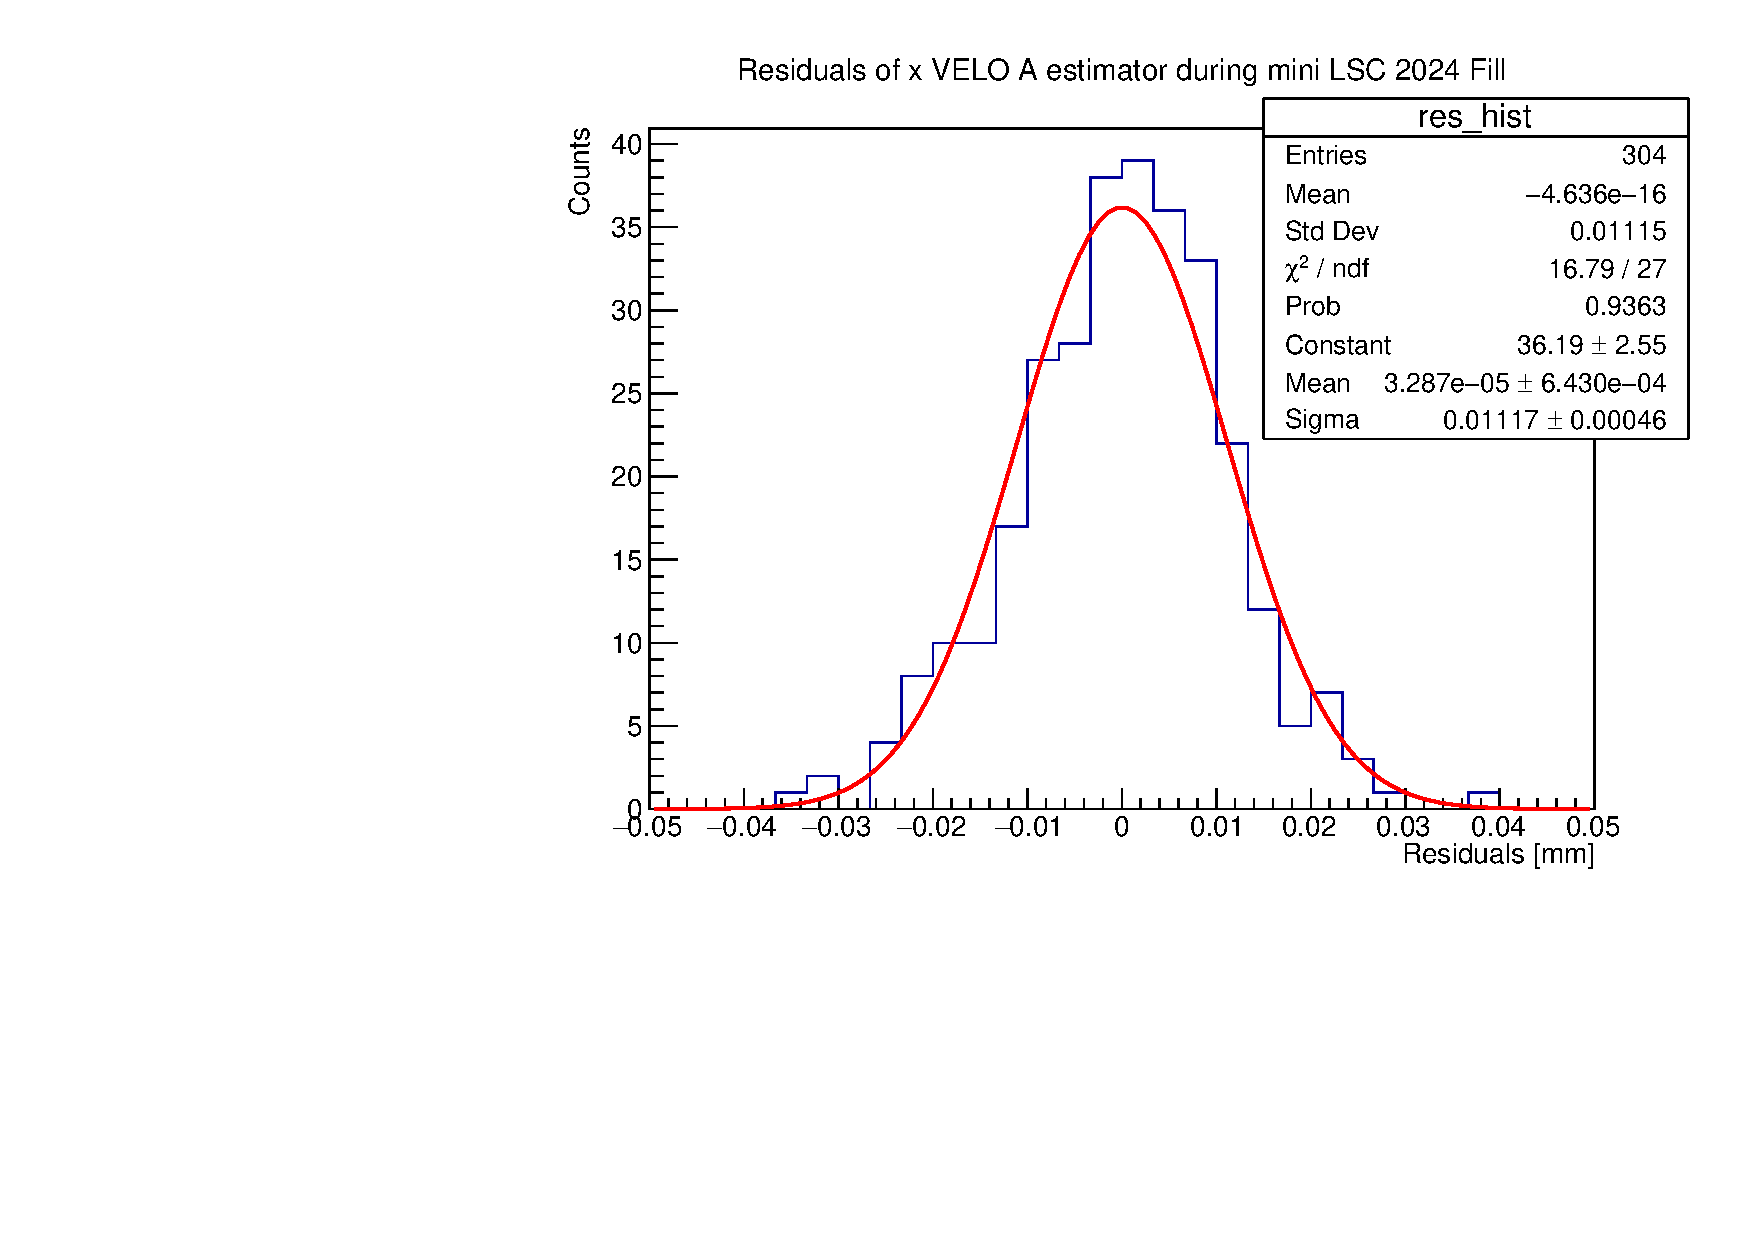
\includegraphics[width=\linewidth]{figures/xVeloA_res_compariosn.pdf}
    \caption{Residuals from the fit of the graph on the left. }\label{fig:xAres_comparison}
    \end{subfigure}
    \caption{$\hat{x}_{A}$ estimator vs monitored position shifts in x component of the A side, alongside the residuals distribution fitted with a Gaussian distribution.}
    \label{fig:xA_comaprison}
\end{figure}
\begin{figure}
    \centering
    \begin{subfigure}{0.48\textwidth}
    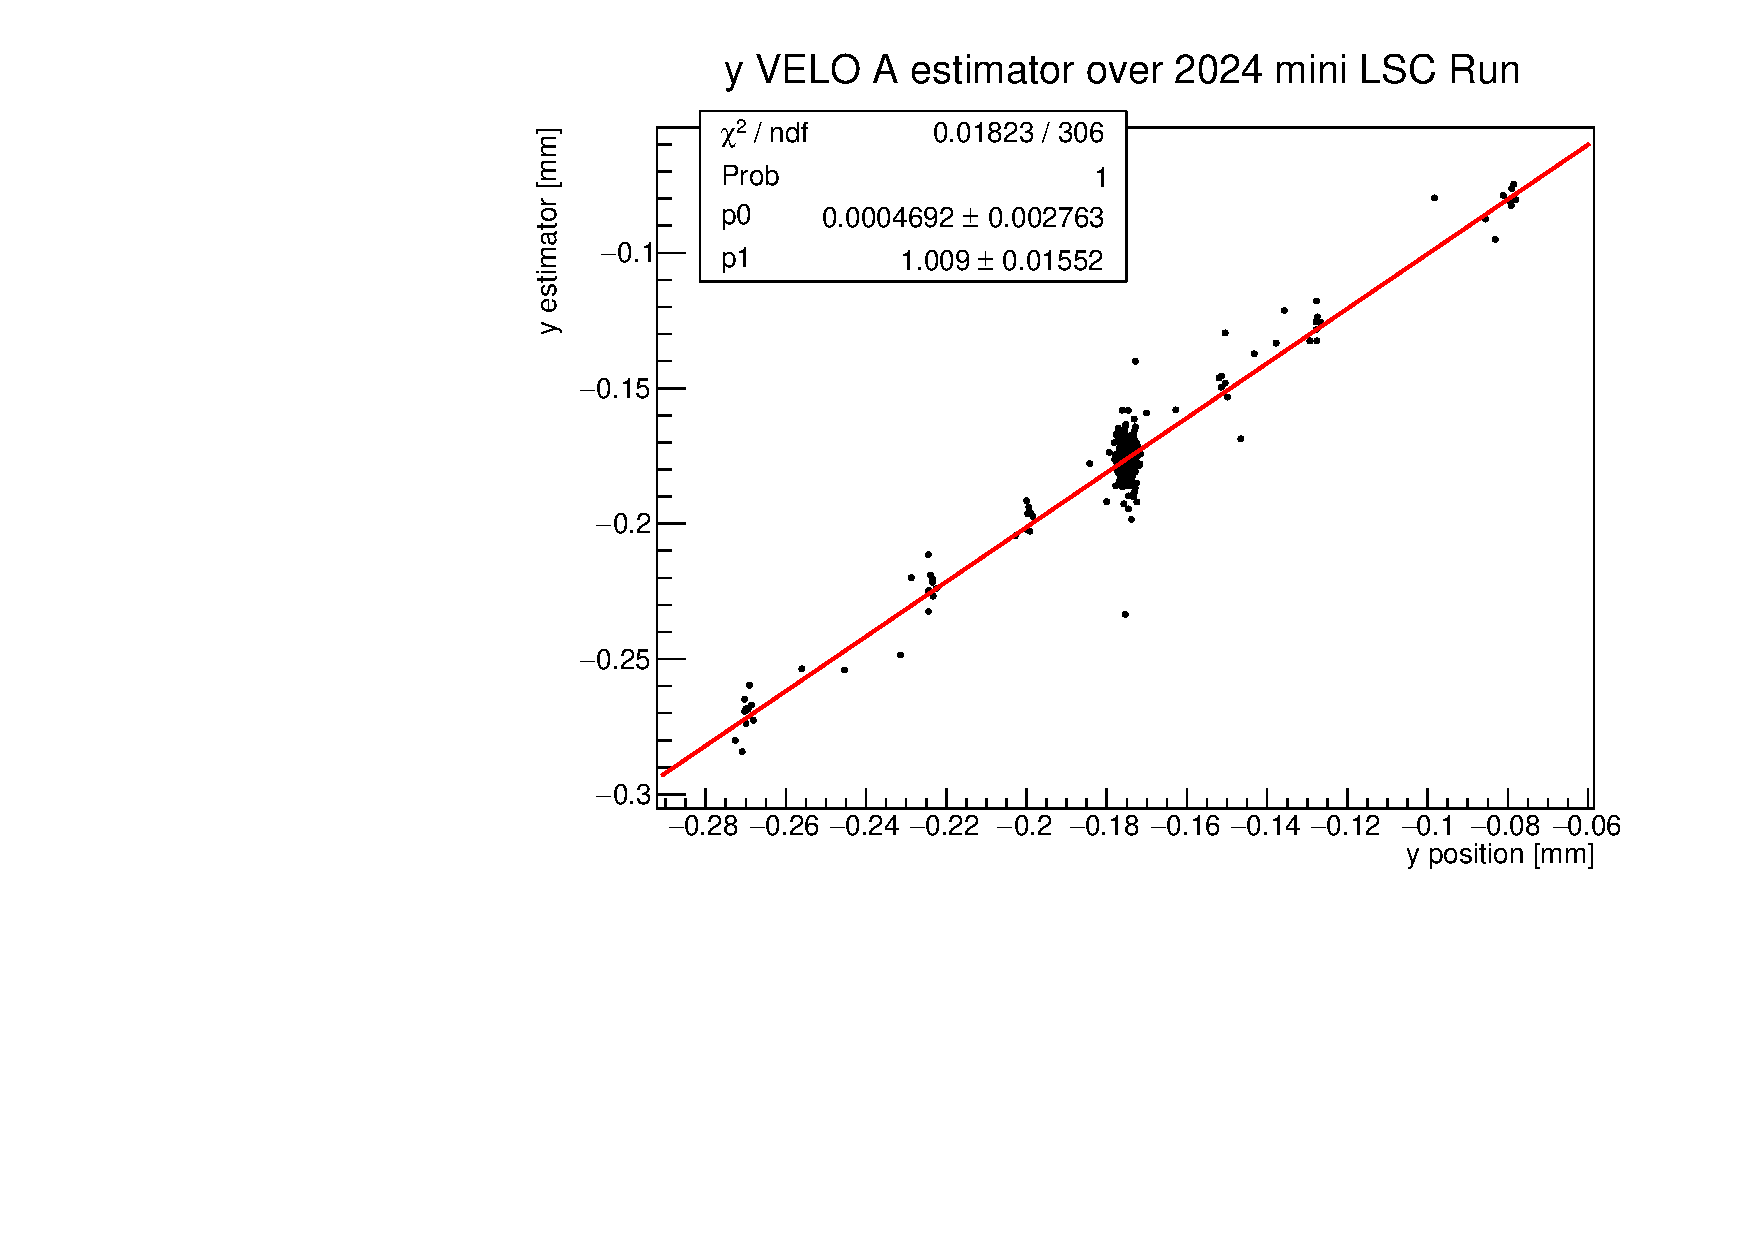
\includegraphics[width=\linewidth]{figures/yVeloA_fit_comparison.pdf}
    \caption{Linear Fit}\label{fig:yAfit_comparison}
    \end{subfigure}
    \begin{subfigure}{0.48\textwidth}
    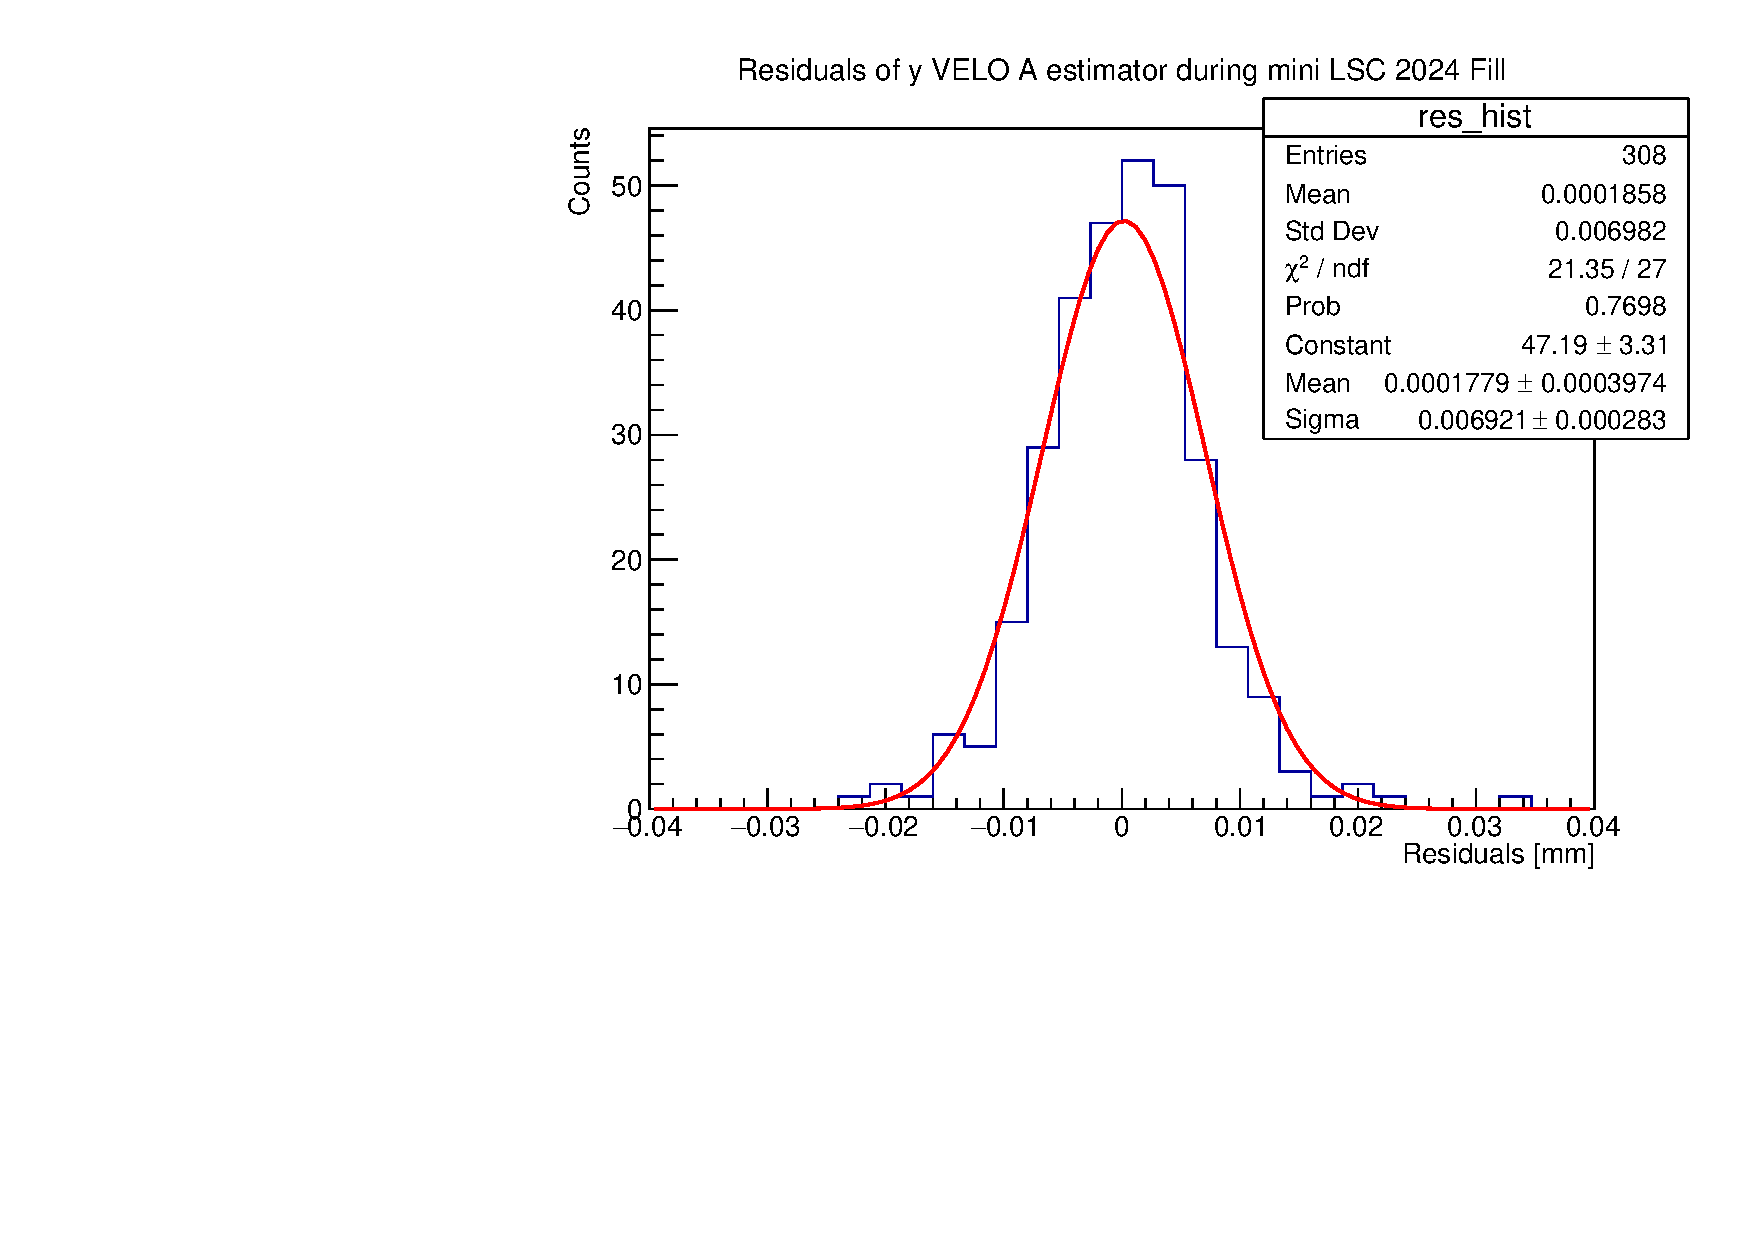
\includegraphics[width=\linewidth]{figures/yVeloA_res_comparison.pdf}
    \caption{Residuals from the fit of the graph on the left. }\label{fig:yAres_comparison}
    \end{subfigure}
    \caption{$\hat{y}_{A}$ estimator vs monitored position shifts in y component of A side, alongside the residuals distribution fitted with a Gaussian distribution.}
    \label{fig:yA_comparison}
\end{figure}

\begin{figure}
    \centering
    \begin{subfigure}{0.48\textwidth}
    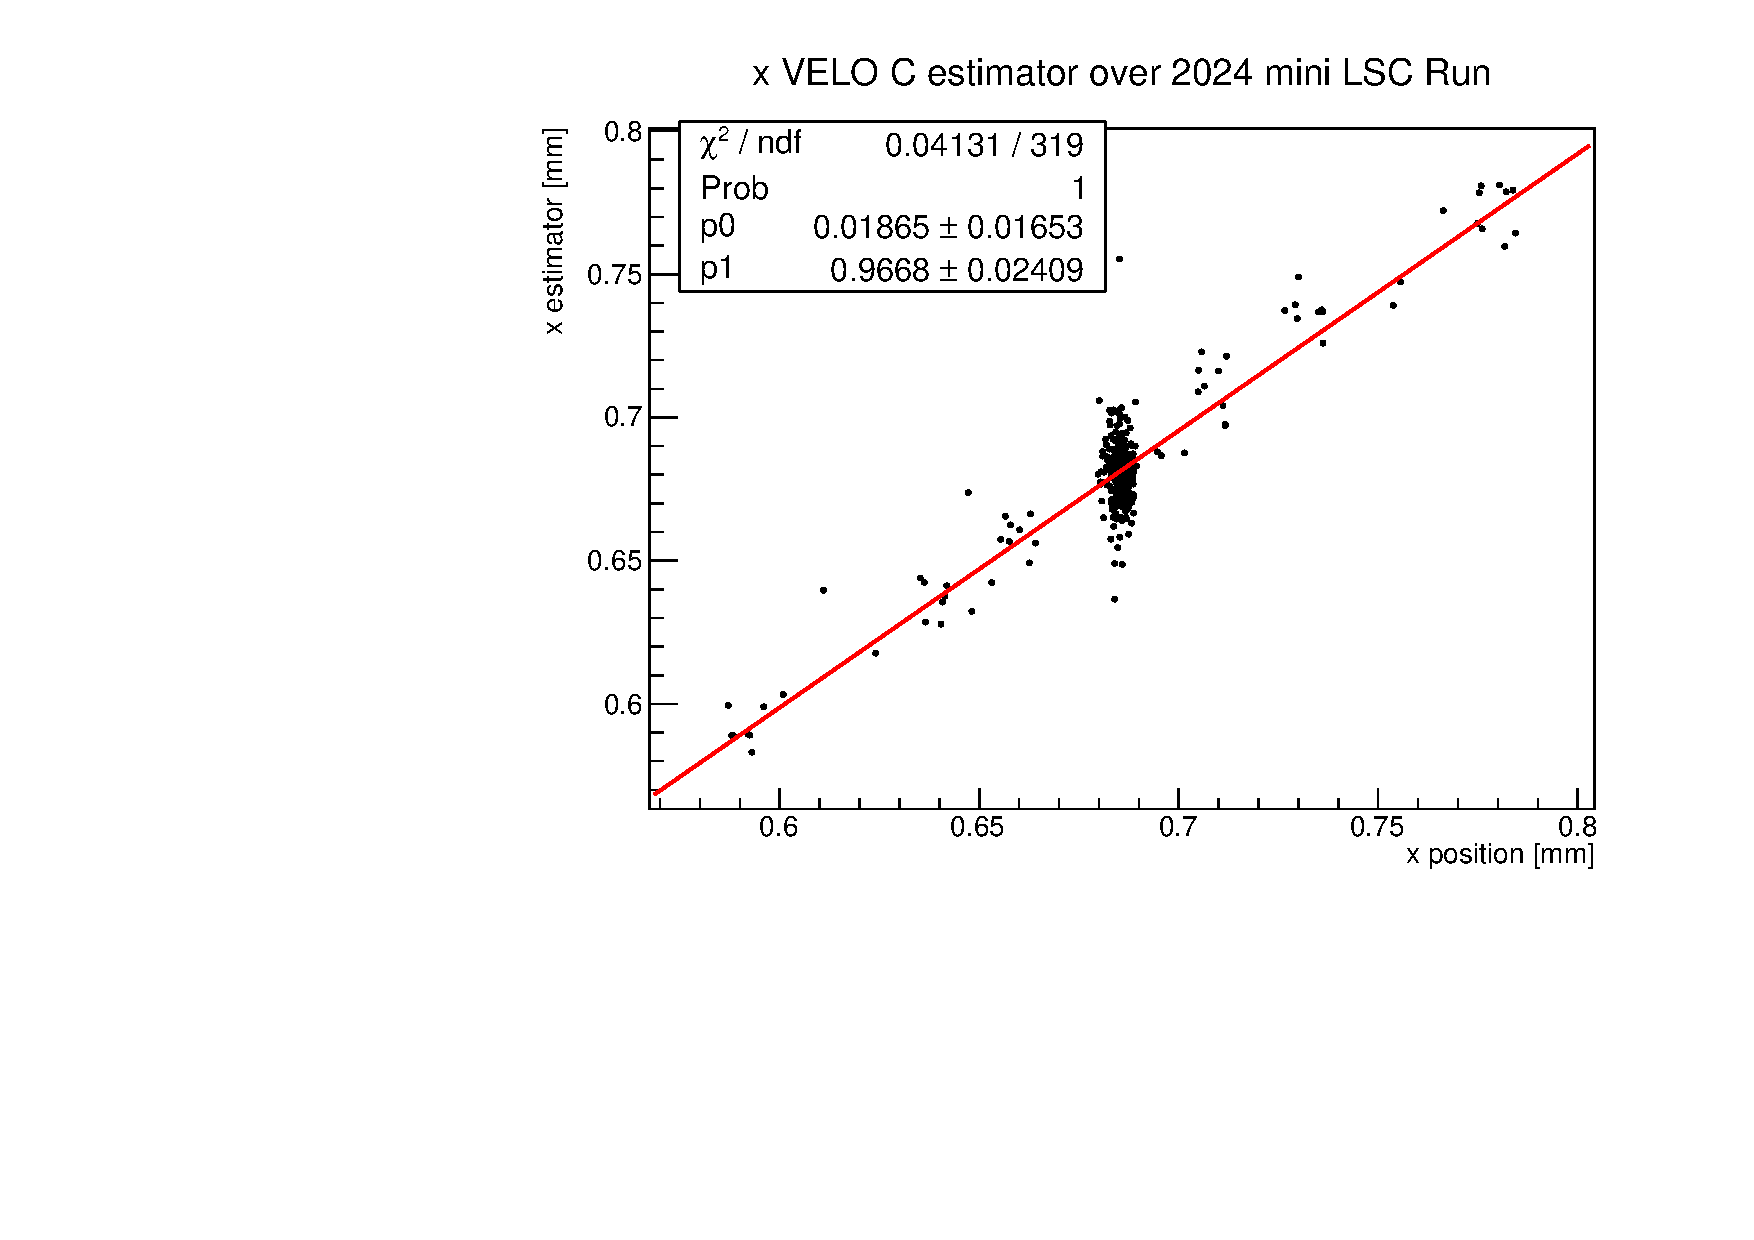
\includegraphics[width=\linewidth]{figures/xVeloC_fit_comparison.pdf}
    \caption{Linear Fit}\label{fig:xCfit_comparison}
    \end{subfigure}
    \begin{subfigure}{0.48\textwidth}
    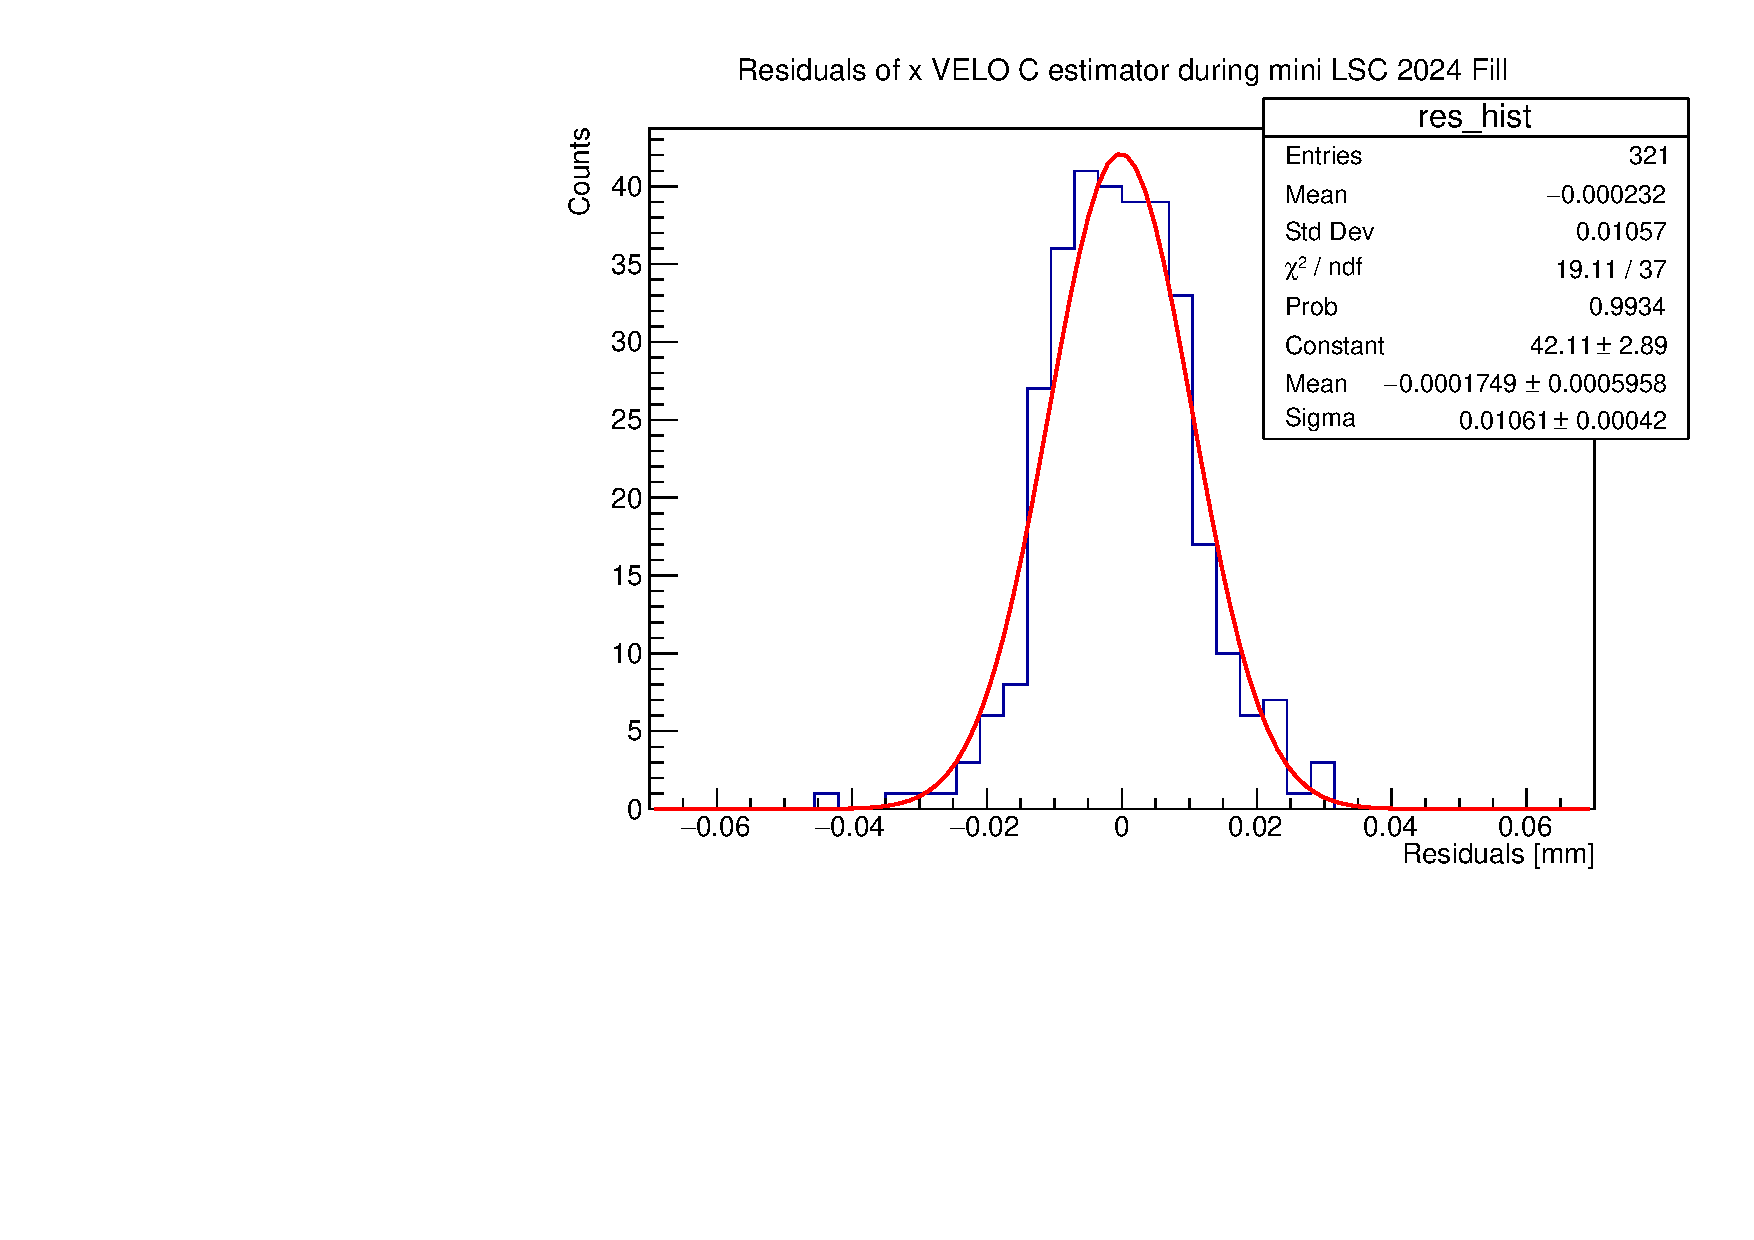
\includegraphics[width=\linewidth]{figures/xVeloC_res_comparison.pdf}
    \caption{Residuals from the fit of the graph on the left. }\label{fig:xCres_comparison}
    \end{subfigure}
    \caption{$\hat{x}_{C}$ estimator vs monitored position shifts in x component of the C side, alongside the residuals distribution fitted with a Gaussian distribution.}
    \label{fig:xC_comaprison}
\end{figure}
\begin{figure}
    \centering
    \begin{subfigure}{0.48\textwidth}
    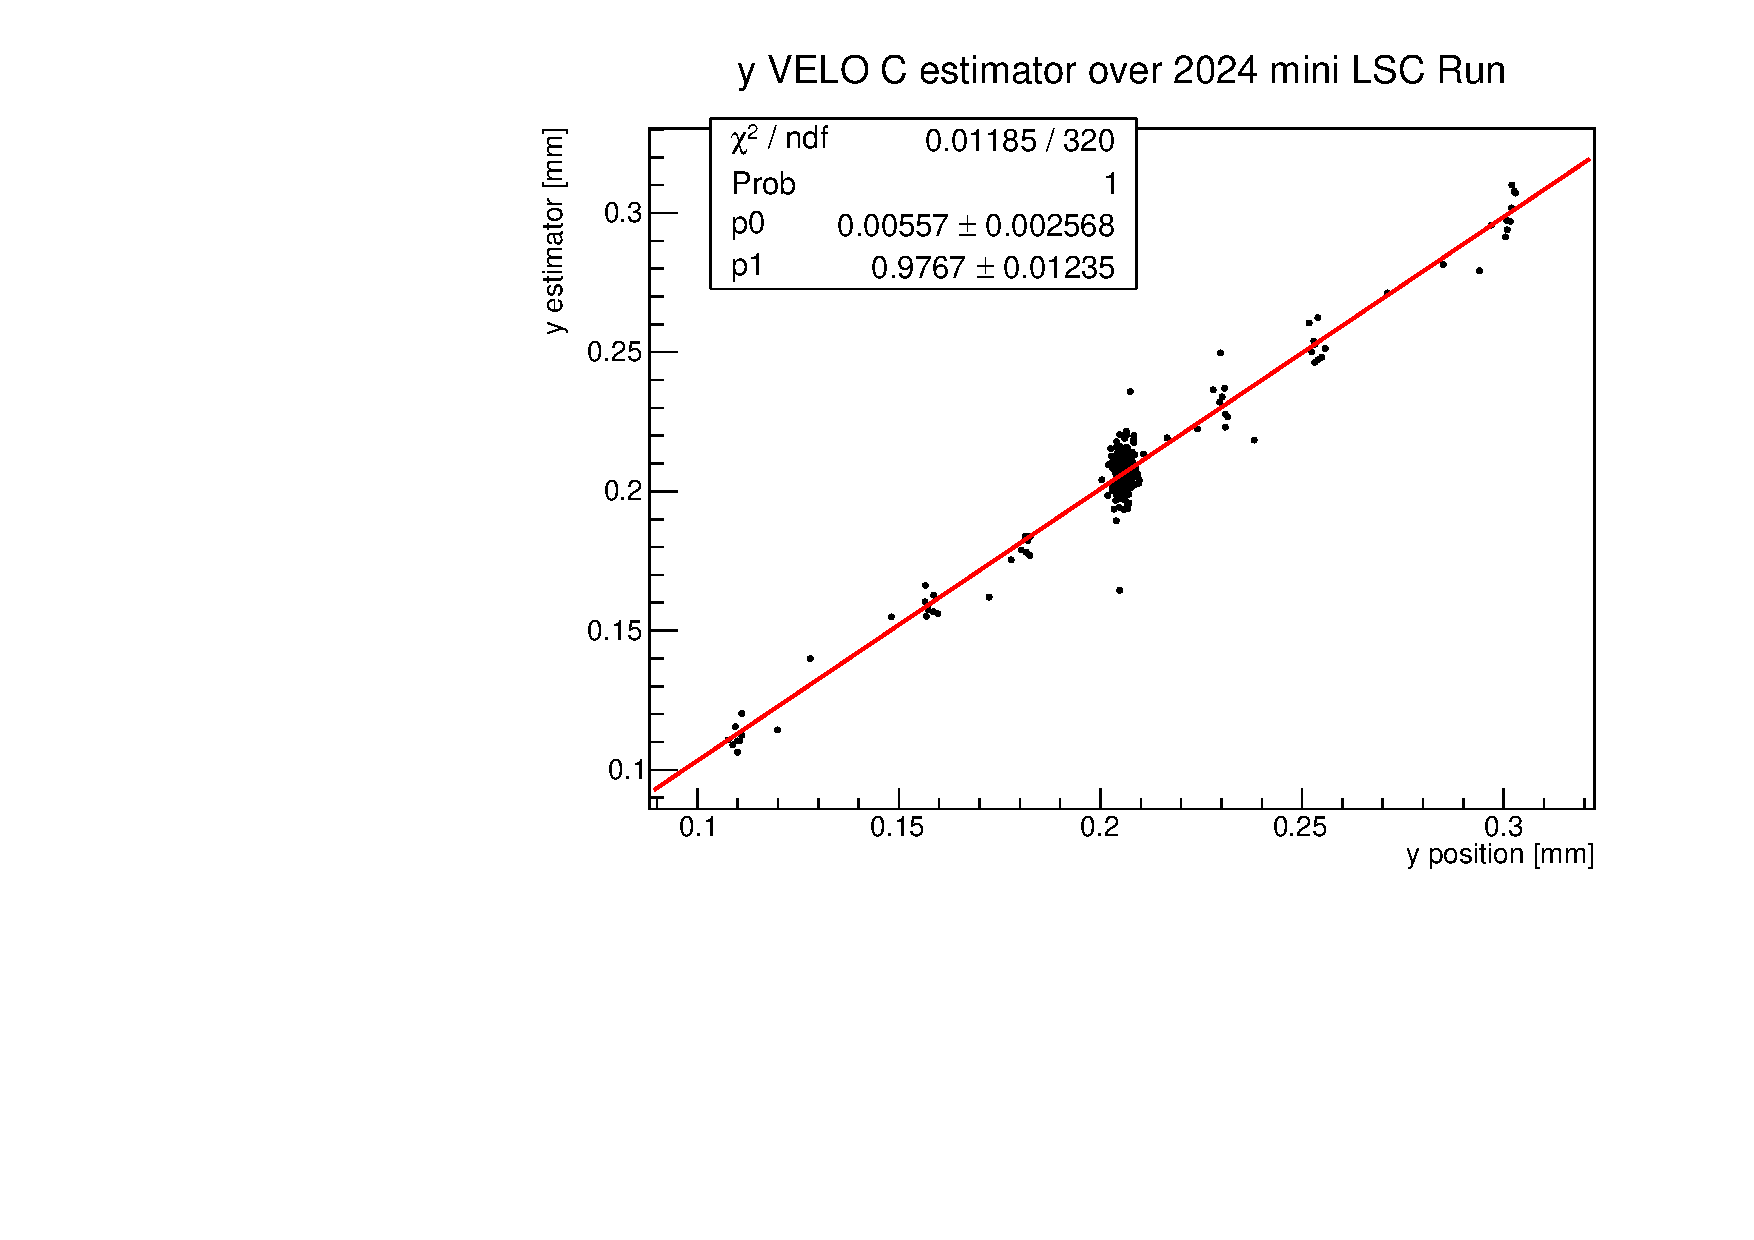
\includegraphics[width=\linewidth]{figures/yVeloC_fit_comparison.pdf}
    \caption{Linear Fit}\label{fig:yCfit_comparison}
    \end{subfigure}
    \begin{subfigure}{0.48\textwidth}
    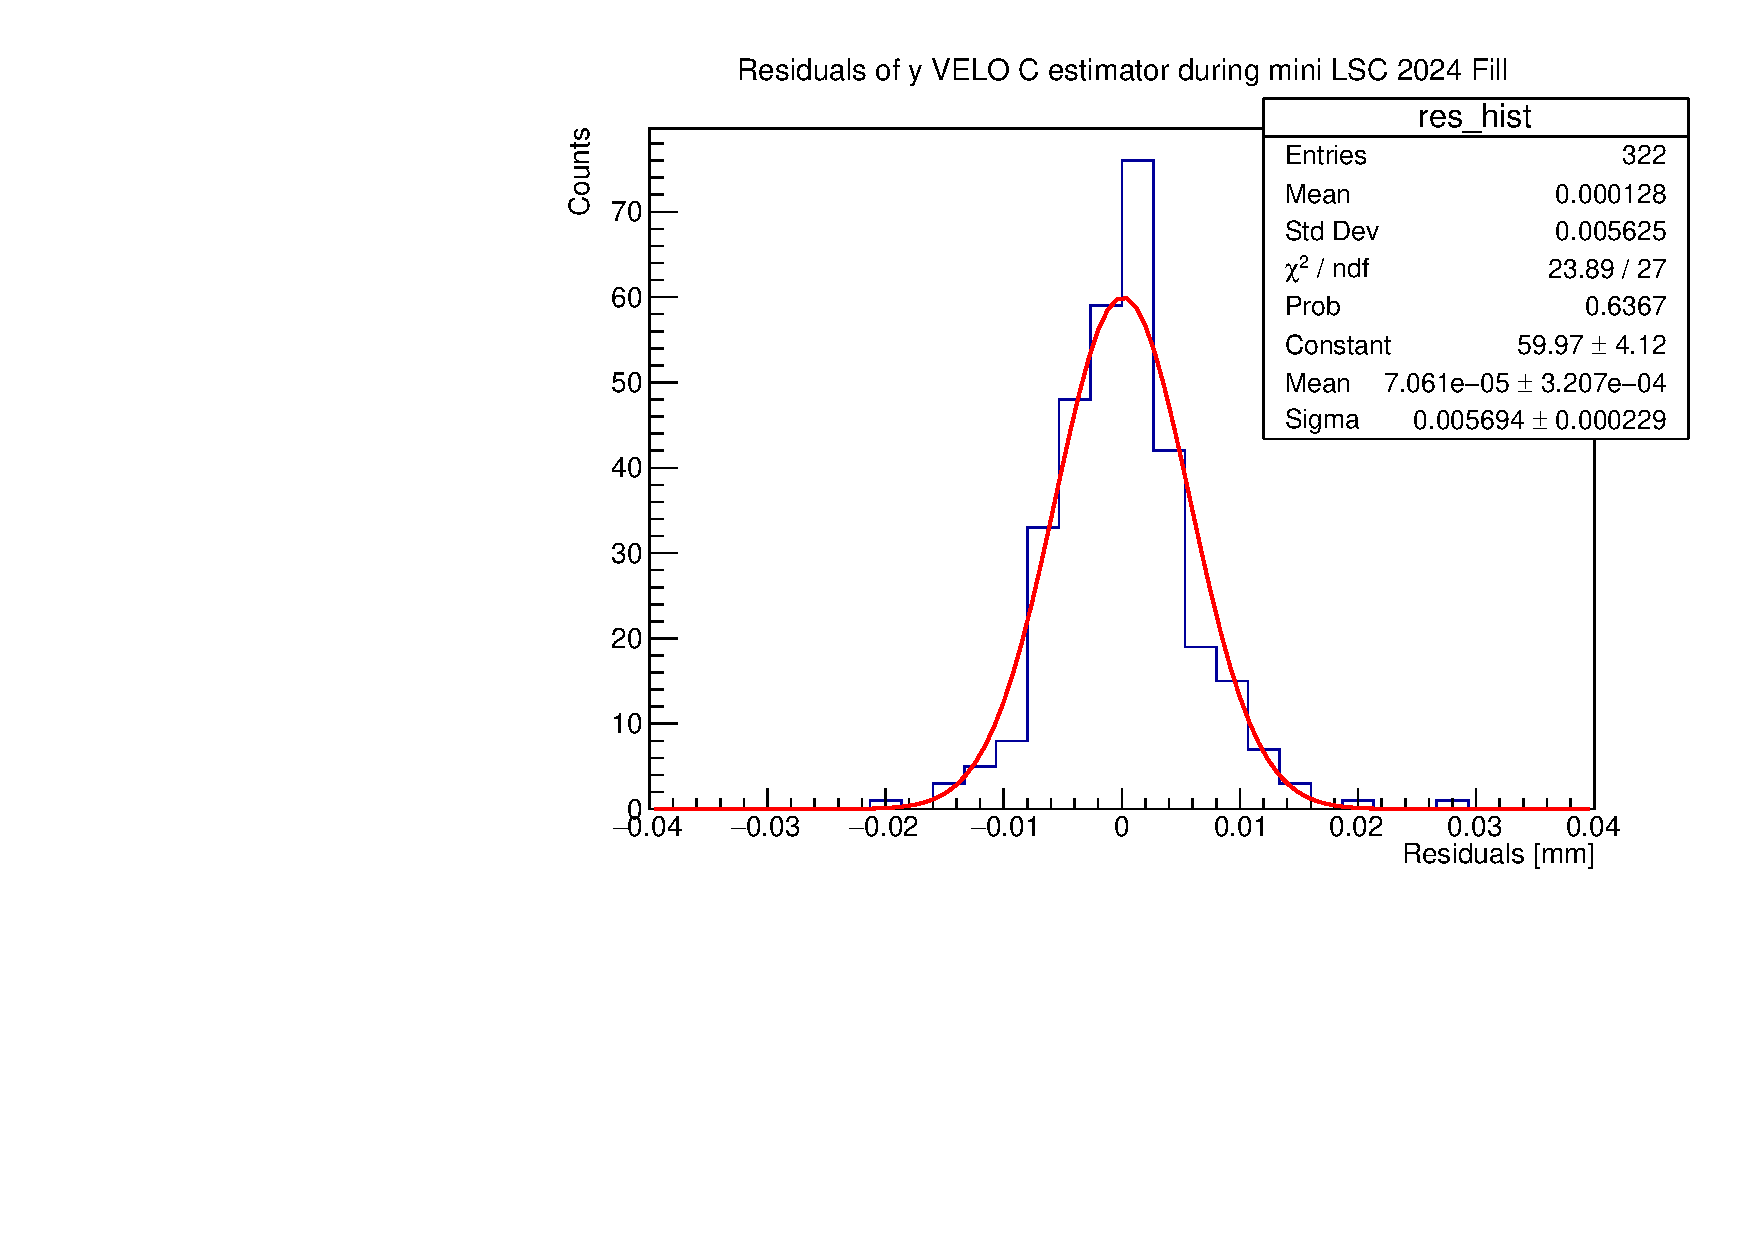
\includegraphics[width=\linewidth]{figures/yVeloC_res_comparison.pdf}
    \caption{Residuals from the fit of the graph on the left. }\label{fig:yCres_comparison}
    \end{subfigure}
    \caption{$\hat{y}_{C}$ estimator vs monitored position shifts in y component of C side, alongside the residuals distribution fitted with a Gaussian distribution.}
    \label{fig:yC_comparison}
\end{figure}

\begin{table}
    \centering
    \begin{tabular}{c|c|c|c|c|c|c}
    variable  & $p0$ & $p1$ & $\sigma_{p0}$ & $\sigma_{p1}$ & distance $p0=0$ [$\sigma$] & distance $p1=1$ [$\sigma$]\\
    \hline
       xA  & -0.017 & 0.962 & 0.011 & 0.024 & 1.5 & 1.6\\
       yA  & 0.00047 & 1.009 & 0.0028 & 0.015 & 0.2 & 0.6 \\
       xC & 0.019 & 0.967 & 0.016 & 0.024 & 1.2 & 1.4\\
       yC & 0.0056 & 0.977 & 0.0026 & 0.012 & 2.1 & 1.9
    \end{tabular}
    \caption{Summary of comparison between estimators and monitored positions by the VELO}
    \label{tab:summary_velo}
\end{table}

Once the calibration performed on the data is validated, we can compare it to the calibration performed in Monte Carlo. As a comparison, we report in Table~\ref{tab:comparison_coeff} the estimated coefficients from both the Monte Carlo and the data, as well as the difference  between the two values expressed in units of the error $\sigma$ of the data-estimated parameters.

\begin{table}
\centering
\begin{tabular}{
c |
c |
c |
c |
c |
c |
c }
 & $a_{\text{MC}}$ & $a_{\text{data}}$ &  $\Delta a$ [$\sigma_a$] & $b_{\text{MC}}$ &  $b_{\text{data}}$ &  $\Delta b$ [$\sigma_b$] \\ \hline
    { xA} &
  { $44.29$} &
  { $43.13\pm1.03$} &
  $1.12$ &%{ $2.7\%$} &
  { $-11.63$} &
  { $-11.91\pm0.27$} &
  $1.04$\\%{ $2.3\%$} \\
    { xC} &
  { $-43.05$} &
  { $-46.62\pm1.26$} &
  $2.83$&%{ $7.6\% $} &
  { $11.99 $} &
  { $13.33\pm0.34$} &
  $3.94$\\%{ $10\%  $} \\
    { yA} &
  { $-43.97$} &
  { $-55.46\pm 1.16$} &
  $9.90$ &%{ $26\%  $} &
  { $0.127 $} &
  { $-0.051\pm0.003$} &
  $59.33$\\%{ $349\% $} \\
    { yC} &
  { $42.77 $} &
  { $43.91\pm0.80 $} &
  $1.41$&%{ $2.6\% $} &
  { $-0.155$} &
  { $0.123\pm0.002 $} &
  $139$%{ $226\% $}
\end{tabular}
\caption{Summary and comparison of coefficients estimated from MC and estimated from data. }\label{tab:comparison_coeff}
\end{table}
This comparison is of great use, as we can see that the calibration for the $x$ estimators are similar one to the other, with the difference not exceeding $4\sigma$. As for the parameters of the $y$ estimators, three of them out of four find themselves in strong disagreement. An explanation for the offsets $b$ could be given by .... 


\section{A testing scenario: monitoring the VELO drift}

